\documentclass[11pt]{article}
\usepackage[margin=1in]{geometry}
\usepackage{booktabs}
\usepackage{graphicx}
\usepackage{amsmath,amssymb}
\usepackage{hyperref}
\usepackage{xcolor}
\usepackage{caption}
\usepackage{subcaption}
\usepackage{array}
\usepackage{multirow}
\usepackage{placeins}

\hypersetup{colorlinks=true, linkcolor=blue, citecolor=blue, urlcolor=blue}

\title{Empirical Analysis of Persuasive Recommendation\\with Endogenous Preference Dynamics:\\[4pt] Evidence from the MIND Dataset}
\author{UBC Gang}
\date{April 2026}

\begin{document}
\maketitle

\begin{abstract}
This report studies whether recommendation systems merely respond to preferences or also help shape them. Using the Microsoft News Dataset (MIND), we analyze large-scale news recommendation data over a 14-day horizon and organize the evidence around four empirical questions. First, is a user's current taste predictive of what they click? Second, does realized consumption alter subsequent taste? Third, how local is persuasion, in the sense that content far from a user's current interests may be hard to move through? Fourth, does mere exposure matter, or is engagement the operative channel?

The main empirical results are sharp. Cosine similarity between a user's estimated taste vector and an article's feature vector strongly predicts clicks, and a simple multinomial logit based only on similarity achieves an AUC of 0.707. In a three-period design, future taste shifts toward what users clicked in the intermediate period, with very strong directional alignment relative to permutation-based null benchmarks. Session-level behavior also exhibits strong self-reinforcement: after a category is clicked, the probability of returning to it in the next session rises substantially.

The most important distinction in the report is between exposure and engagement. Content that is shown and clicked predicts subsequent taste growth in that category, whereas content that is shown but ignored does not. In fact, ignored exposure is associated with subsequent movement \emph{away} from the exposed category relative to a never-shown baseline. This pattern is economically important, statistically precise, and present across almost all categories. Taken together, the evidence supports a model in which recommendation affects preferences primarily through \emph{clicked} content, subject to a local persuasion constraint and heterogeneous category-level dynamics.
\end{abstract}

% TODO (meeting note): The backfire finding might be relevant to fatigue or Berlyne's two-factor theory — discuss in a meeting.

%======================================================================
\section{Empirical Questions and Roadmap}
%======================================================================

The report is organized to answer a sequence of empirical questions that correspond directly to the theoretical ingredients of a persuasive recommendation model.

Section~\ref{sec:utility} asks whether a user's estimated taste vector has predictive power for individual click decisions. This is the empirical foundation for representing utility as an inner product between user taste and article features.

Section~\ref{sec:taste} asks whether tastes evolve in the direction of realized consumption, rather than simply reflecting the platform's assortment. This section combines session-level evidence, a three-period design, and regressions that control for what the platform chose to show.

Section~\ref{sec:persuasion} and Section~\ref{sec:tradeoff} study how far recommendation can reach. If users mainly click content close to their current taste, then persuasion is local, and the platform faces an exploitation--exploration tradeoff between high-probability clicks and larger potential taste updates.

Section~\ref{sec:assortment} and Section~\ref{sec:exposure} then ask whether the relevant mechanism is exposure itself or engagement with exposed content. These sections are central for the optimization problem: if ignored exposure has little value, or even backfires, then the platform should optimize for click-inducing exposure rather than raw impression volume.

Finally, Section~\ref{sec:fine} documents richer structure in the dynamics, including diversification, compounding, category stickiness, and partial mean reversion. These patterns matter because a realistic optimization model should not treat all categories or all clicks as interchangeable.

%======================================================================
\section{Data and Design}
%======================================================================

\subsection{Datasets}

We use both publicly released versions of the Microsoft News Dataset (MIND), summarized in Table~\ref{tab:datasets}. MINDlarge is the main dataset for the dynamic analyses because its longer horizon supports the three-period design introduced below. MINDsmall is used primarily as a robustness check and for short-horizon replication.

\begin{table}[ht]
\centering
\caption{MIND dataset summary. Each impression contains a user's click history and a list of shown articles with binary click labels.}
\label{tab:datasets}
\begin{tabular}{llccc}
\toprule
Dataset & Split & Dates & Impressions & Users \\
\midrule
\multirow{2}{*}{MINDsmall} & Train & Nov 9--14 & 156,965 & \multirow{2}{*}{94,057} \\
 & Dev & Nov 15 & 73,152 & \\
\midrule
\multirow{3}{*}{MINDlarge} & Train & Nov 9--14 & 2,232,748 & \multirow{3}{*}{${\sim}$1M} \\
 & Dev & Nov 15 & 376,471 & \\
 & Test & Nov 16--22 & 2,370,727 & \\
\bottomrule
\end{tabular}
\end{table}
\FloatBarrier

An \emph{impression} is a recommendation opportunity: it contains the user's accumulated click history up to that point and a slate of candidate articles, each with a binary click label when labels are available. The MINDlarge test split does not provide click labels directly, but it does preserve the evolving click history, which lets us infer the articles clicked in Period~3 by comparing the history before and after the test window. Articles are assigned to 15 broad categories and 285 subcategories. The large and small versions contain 104,151 and 51,282 unique articles, respectively.

\subsection{Notation and representations}
\label{sec:notation}

Let $i$ index users, $j$ index articles, and $k$ index content categories. Each article $j$ is represented by a feature vector $\mathbf{v}_j$. We use two alternative feature constructions.

The first is a 285-dimensional one-hot encoding of the MIND subcategory. This representation has full coverage and is the baseline representation throughout the report. The second is a 100-dimensional dense embedding obtained by averaging the pre-trained Wikidata entity embeddings associated with the article. This representation is available for 73.7\% of articles and is used as a secondary validity check.

For each user $i$, the latent taste vector $\boldsymbol{\theta}_i$ is estimated as the mean feature vector of the articles clicked by that user up to the relevant point in time. Thus, $\boldsymbol{\theta}_i$ is not an arbitrary parameter: it is an empirical summary of the user's revealed interests.

Several later analyses are conducted at the category level rather than the article-feature level. In those analyses, we write $\boldsymbol{\theta}_i \in \mathbb{R}^{14}$ for the vector of category shares, where $\theta_{i,k}$ is the fraction of user $i$'s clicks in category $k$. The kids category is omitted from this representation because it has fewer than 100 clicks in total; the remaining 14 categories account for more than 99.9\% of all observed clicks. When we study impression-level assortment composition in Section~\ref{sec:assortment}, we retain all 15 categories because those tests do not require a stable user-level taste vector for each category.

\subsection{Three-period design}
\label{sec:three_period_design}

The dynamic analyses use a three-period design built from the 14-day MINDlarge window. Period~1 (P1, Nov~9--11) is the \emph{baseline period} and is used to estimate initial taste. Period~2 (P2, Nov~12--15) is the \emph{intermediate period} in which we observe both exposure and consumption. Period~3 (P3, Nov~16--22) is the \emph{future period} and is used to measure subsequent taste after the P2 recommendation and click history.

This partition is important for interpretation. P1 gives a pre-period measure of taste, P2 contains the potentially persuasive experiences, and P3 provides the post-period outcome. Throughout the report, $\boldsymbol{\theta}_i^{(\mathrm{P}t)}$ denotes user $i$'s estimated taste vector in period $t$.

\subsection{Analysis sample}

Different analyses require different support conditions, so the effective sample varies across sections. Sections~\ref{sec:utility} through \ref{sec:assortment} use a working sample of 50,000 users, corresponding to 187,088 impressions and 7.15 million article-level observations. The three-period taste-shift tests use 143,574 users with at least two clicks in each period so that both baseline and future taste vectors are well defined. The exposure-versus-engagement analysis uses 145,985 users with at least two clicks in P1 and P2, at least five shown articles in P2, and at least two inferred clicks in P3. Unless noted otherwise, all reported percentages and correlations are computed within the relevant analysis sample. The unconditional article-level click-through rate in the working sample is 4.07\%.


%======================================================================
\section{Inner-Product Utility}
\label{sec:utility}
%======================================================================

This section evaluates the most basic behavioral assumption in the model: users are more likely to click articles whose features are better aligned with their current taste. Formally, the model writes user $i$'s utility from article $j$ as
\[
u_{ij} = \langle \boldsymbol{\theta}_i,\mathbf{v}_j\rangle,
\]
where $\boldsymbol{\theta}_i$ is the user's estimated taste vector and $\mathbf{v}_j$ is the article feature vector. Because cosine similarity is the scale-free version of the inner product, the empirical implication is simple: higher similarity should be associated with a higher click-through rate (CTR), where CTR is the fraction of shown articles that are clicked.

To test this implication nonparametrically, we compute
\[
\text{sim}_{ij} = \cos(\boldsymbol{\theta}_i,\mathbf{v}_j)
\]
for each user--article pair and sort observations into similarity quintiles. Table~\ref{tab:sim_quintile} reports the resulting CTR profile.

\begin{table}[ht]
\centering
\caption{CTR by cosine-similarity quintile. Higher similarity between user taste and article features predicts higher click-through rates.}
\label{tab:sim_quintile}
\begin{tabular}{cccc}
\toprule
Sim quintile & Mean similarity & CTR & $N$ \\
\midrule
0 (lowest) & 0.000 & 2.86\% & 4,290,400 \\
1 & 0.070 & 4.18\% & 715,294 \\
2 & 0.163 & 4.94\% & 715,077 \\
3 & 0.298 & 5.95\% & 715,185 \\
4 (highest) & 0.587 & 8.49\% & 714,526 \\
\bottomrule
\end{tabular}
\end{table}
\FloatBarrier

Table~\ref{tab:sim_quintile} shows a strong monotone pattern: CTR rises from 2.86\% in the lowest similarity quintile to 8.49\% in the highest. The table is important because it is purely descriptive and does not rely on any modeling assumptions beyond the construction of $\boldsymbol{\theta}_i$ and $\mathbf{v}_j$.

To summarize the relationship with a single statistic, we also compute the point-biserial correlation between $\text{sim}_{ij}$ and the binary click indicator. This statistic measures the association between a continuous regressor and a binary outcome. Using subcategory embeddings, the correlation is $r = 0.095$ ($p < 10^{-300}$); using entity embeddings, it is $r = 0.055$ ($p < 10^{-300}$). The magnitudes are modest, which is expected in noisy behavioral data, but the sign is stable and the effect is highly precisely estimated.

A sharper test treats each impression as a discrete-choice set. For an impression showing articles $j=1,\ldots,J$, we estimate a multinomial logit,
\[
P(\text{click }j) = \frac{\exp(\beta\,\text{sim}_{ij})}{\sum_{k=1}^{J}\exp(\beta\,\text{sim}_{ik})},
\]
where $\beta$ is fitted by maximum likelihood. Table~\ref{tab:auc} reports out-of-sample AUC on 100,000 held-out impressions.

\begin{table}[ht]
\centering
\caption{Click prediction accuracy (AUC) by predictor. The MNL uses only similarity constructed from subcategory-based article features.}
\label{tab:auc}
\begin{tabular}{lc}
\toprule
Predictor & AUC \\
\midrule
Subcategory cosine similarity & 0.613 \\
Entity cosine similarity & 0.576 \\
Combined & 0.618 \\
MNL (subcategory features only) & \textbf{0.707} \\
\bottomrule
\end{tabular}
\end{table}
\FloatBarrier

The main message from Table~\ref{tab:auc} is that even a very sparse preference representation contains substantial predictive content. The MNL reaches an AUC of 0.707 using only similarity based on subcategory features, without article text, recency controls, or feed-position information. This does not prove that the inner-product model is complete, but it does show that it captures an economically meaningful part of click behavior. The controlled regressions in Section~\ref{sec:regression} will strengthen this conclusion by showing that historical taste continues to matter even after we control directly for the platform's assortment composition.


%======================================================================
\section{Taste Dynamics}
\label{sec:taste}
%======================================================================

\subsection{Self-reinforcement}

The first dynamic question is whether taste exhibits short-run reinforcement. We split each user's activity into daily sessions and, for each category $c$, compare the probability of clicking $c$ in session $t+1$ after the user did versus did not click $c$ in session $t$. Formally, the percentage lift is
\[
\text{Lift}_c = \frac{P(c\text{ clicked at }t{+}1\mid c\text{ clicked at }t)-P(c\text{ clicked at }t{+}1\mid c\text{ not clicked at }t)}{P(c\text{ clicked at }t{+}1\mid c\text{ not clicked at }t)}.
\]
Table~\ref{tab:selfreinforcement} reports these transition statistics category by category.

\begin{table}[ht]
\centering
\caption{Session-level self-reinforcement by category. Lift measures the percentage increase in next-session click probability after clicking a category versus not clicking it.}
\label{tab:selfreinforcement}
\small
\begin{tabular}{lcccr}
\toprule
Category & $P(\text{next} \mid \text{click})$ & $P(\text{next} \mid \text{no click})$ & Lift & $p$-value \\
\midrule
autos & 0.127 & 0.023 & $+448\%$ & $< 10^{-300}$ \\
video & 0.068 & 0.019 & $+254\%$ & $< 10^{-300}$ \\
foodanddrink & 0.118 & 0.036 & $+232\%$ & $< 10^{-300}$ \\
weather & 0.061 & 0.024 & $+154\%$ & $< 10^{-143}$ \\
health & 0.080 & 0.034 & $+132\%$ & $< 10^{-300}$ \\
travel & 0.058 & 0.026 & $+127\%$ & $< 10^{-234}$ \\
entertainment & 0.077 & 0.035 & $+122\%$ & $< 10^{-300}$ \\
movies & 0.031 & 0.014 & $+123\%$ & $< 10^{-71}$ \\
sports & 0.243 & 0.113 & $+114\%$ & $< 10^{-300}$ \\
lifestyle & 0.193 & 0.105 & $+84\%$ & $< 10^{-300}$ \\
tv & 0.068 & 0.044 & $+53\%$ & $< 10^{-129}$ \\
finance & 0.116 & 0.080 & $+45\%$ & $< 10^{-184}$ \\
news & 0.353 & 0.245 & $+44\%$ & $< 10^{-300}$ \\
music & 0.077 & 0.060 & $+29\%$ & $< 10^{-54}$ \\
\midrule
\textbf{Overall} & \textbf{0.184} & \textbf{0.054} & $\boldsymbol{+243\%}$ & $< 10^{-300}$ \\
\bottomrule
\end{tabular}
\end{table}
\FloatBarrier

Table~\ref{tab:selfreinforcement} shows positive reinforcement in every category. The overall lift is $+243\%$, which means that the probability of returning to a category in the next session is 3.4 times as large after a click as after a non-click. The category-level heterogeneity is also informative. Niche categories such as autos and video have the largest proportional lifts because their baseline re-click probabilities are low. Broad categories such as news have smaller percentage lifts but still large absolute differences. The empirical takeaway is not merely that tastes are persistent; it is that recently consumed categories become temporarily more behaviorally salient, which is exactly the local updating force assumed in many dynamic recommendation models.

\subsection{Three-period taste shift}
\label{sec:three_period}

The session analysis above is short run. The next question is whether tastes \emph{move} over a longer horizon in the direction of what users consume. Using the three-period design from Section~\ref{sec:three_period_design}, we define the net taste change for user $i$ as
\[
\Delta\boldsymbol{\theta}_i = \boldsymbol{\theta}_i^{(\mathrm{P3})} - \boldsymbol{\theta}_i^{(\mathrm{P1})}.
\]
We then compare this vector to consumption vectors constructed from clicked content. The central object is the cosine alignment between a taste-change vector and a period-specific consumption vector: a positive cosine means that taste moved toward what the user consumed; a value near zero means no directional relation; a negative value means movement away. For compactness, let
\[
\Delta\boldsymbol{\theta}_i^{12}=\boldsymbol{\theta}_i^{(\mathrm{P2})}-\boldsymbol{\theta}_i^{(\mathrm{P1})},
\qquad
\Delta\boldsymbol{\theta}_i^{13}=\boldsymbol{\theta}_i^{(\mathrm{P3})}-\boldsymbol{\theta}_i^{(\mathrm{P1})},
\]
and let $\mathbf{c}_i^{(\mathrm{P}t)}$ denote the consumption vector formed from user $i$'s clicked articles in period $t$.

Table~\ref{tab:taste_alignment} reports three comparisons for the 143,574 users with at least two clicks in each period: a placebo alignment using earlier consumption, the main alignment with P2 consumption, and an alignment with pooled P1+P2 consumption.

\begin{table}[ht]
\centering
\caption{Cosine alignment between taste-change vectors and consumption vectors. Future taste change aligns strongly with intermediate-period consumption.}
\label{tab:taste_alignment}
\begin{tabular}{lccc}
\toprule
Alignment test & Mean $\cos$ & $t$-stat & $p$-value \\
\midrule
Placebo: $\cos(\Delta\boldsymbol{\theta}^{12}, \mathbf{c}^{(\mathrm{P1})})$ & $-0.008$ & $-8.1$ & $4 \times 10^{-16}$ \\
Main: $\cos(\Delta\boldsymbol{\theta}^{13}, \mathbf{c}^{(\mathrm{P2})})$ & $\boldsymbol{+0.360}$ & $\boldsymbol{429}$ & $\boldsymbol{< 10^{-300}}$ \\
Pooled: $\cos(\Delta\boldsymbol{\theta}^{13}, \mathbf{c}^{(\mathrm{P1})}{+}\mathbf{c}^{(\mathrm{P2})})$ & $+0.397$ & $501$ & $< 10^{-300}$ \\
\bottomrule
\end{tabular}
\end{table}
\FloatBarrier

Table~\ref{tab:taste_alignment} is the main evidence that taste drift follows realized consumption rather than arbitrary time trends. The placebo row is near zero and slightly negative, whereas the alignment with P2 consumption is strongly positive at $+0.360$. A permutation test with 1,000 shuffles yields a null mean of essentially zero and a $z$-score of 515, so the observed directional alignment is far outside what would arise from random reassignment. In the shorter 7-day MINDsmall window, the same statistic is $-0.012$ and insignificant. The contrast is useful: the dynamic effect appears to be real but cumulative, and the shorter sample is simply too short to detect it cleanly.
\paragraph{Entropy.} Self-reinforcement raises a natural concern: if clicking a category makes future clicks in that category more likely, do users narrow into a filter bubble? We measure taste concentration using Shannon entropy $H(\boldsymbol{\theta}_i) = -\sum_k \theta_{i,k} \log_2 \theta_{i,k}$, where higher entropy means a more dispersed taste distribution and lower entropy means concentration in fewer categories. Table~\ref{tab:entropy} tracks entropy across the three periods.
\begin{table}[ht]
\centering
\caption{Entropy trajectory across periods. Most users diversify; only 9.3\% are more focused in P3 than in P1.}
\label{tab:entropy}
\begin{tabular}{lcccc}
\toprule
Period & Mean entropy & $\Delta$ from P1 & $t$-stat & More focused \\
\midrule
P1 (Nov 9--11) & 1.352 bits & --- & --- & --- \\
P2 (Nov 12--15) & 1.590 bits & $+0.238$ & $116$ & 34.1\% \\
P3 (Nov 16--22) & 2.047 bits & $+0.678$ & $474$ & 9.3\% \\
\bottomrule
\end{tabular}
\end{table}
\FloatBarrier

Table~\ref{tab:entropy} shows that reinforcement does not mechanically imply narrowing. Mean entropy rises from 1.352 bits in P1 to 2.047 bits in P3, and only 9.3\% of users are more concentrated in P3 than in P1. The relevant distinction is between \emph{within-category reinforcement} and \emph{across-category diversification}. Users can become more likely to return to categories they recently consumed while still broadening the overall set of categories they touch. A model that only allows one of these forces would miss an important empirical feature of the data.
\paragraph{Transition matrix.} If users diversify on average, where does the new taste go? For each user's P1 dominant category, Table~\ref{tab:transition} shows the distribution of P3 clicks across categories.

\begin{table}[ht]
\centering
\caption{Transition matrix: P1 dominant category $\to$ P3 click distribution (143,574 users). Diagonal entries (bold) show self-reinforcement. Row sums $< 1$ because 5 minor categories are omitted from columns.}
\label{tab:transition}
\small
\setlength{\tabcolsep}{3.5pt}
\begin{tabular}{l|cccccccccc}
\toprule
& news & sports & fin. & life. & health & trav. & food & autos & ent. & video \\
\midrule
news & \textbf{.46} & .12 & .07 & .08 & .03 & .03 & .03 & .02 & .02 & .02 \\
sports & .17 & \textbf{.44} & .06 & .06 & .02 & .03 & .03 & .02 & .02 & .01 \\
finance & .23 & .12 & \textbf{.26} & .10 & .04 & .03 & .04 & .02 & .02 & .02 \\
lifestyle & .20 & .08 & .05 & \textbf{.33} & .04 & .03 & .04 & .01 & .04 & .02 \\
health & .19 & .09 & .06 & .13 & \textbf{.24} & .03 & .04 & .02 & .03 & .02 \\
travel & .16 & .08 & .07 & .10 & .04 & \textbf{.28} & .04 & .03 & .03 & .02 \\
food & .18 & .08 & .06 & .13 & .05 & .04 & \textbf{.26} & .02 & .03 & .01 \\
autos & .19 & .11 & .08 & .08 & .04 & .04 & .04 & \textbf{.26} & .03 & .02 \\
ent. & .18 & .09 & .06 & .13 & .05 & .03 & .04 & .01 & \textbf{.21} & .02 \\
video & .20 & .06 & .05 & .10 & .03 & .03 & .03 & .02 & .02 & \textbf{.35} \\
\bottomrule
\end{tabular}
\end{table}
\FloatBarrier

Table~\ref{tab:transition} explains \emph{where} diversification goes. The diagonal entries capture persistence, and they are strongest for the broad categories news and sports. The off-diagonal entries show that drift is highly directional rather than diffuse. Many initial categories feed disproportionately into news and sports, while much smaller flows move into categories such as travel or autos. This matters for theory because it means that a category-to-category transition kernel cannot be treated as symmetric or exchangeable across categories.
\subsection{Controlled regression}
\label{sec:regression}

A key identification concern is that users can only click what the platform chooses to show. To separate latent preference from assortment composition, we run the category-level regression
\[
\text{click\_frac}_{u,c}
=
\beta_0
+
\beta_1\,\text{hist\_frac}_{u,c}
+
\beta_2\,\text{shown\_frac}_{u,c}
+
\varepsilon_{u,c},
\]
where $\text{click\_frac}_{u,c}$ is user $u$'s realized click share in category $c$, $\text{hist\_frac}_{u,c}$ is the historical taste share in that category, and $\text{shown\_frac}_{u,c}$ is the share of displayed articles in that category. The coefficient $\beta_1$ asks whether history predicts future clicking \emph{holding fixed what the algorithm displayed}. Table~\ref{tab:controlled_reg} reports the estimates for both MINDsmall and MINDlarge.

\begin{table}[ht]
\centering
\caption{Controlled regression of click fraction on historical taste and algorithmic assortment. Historical taste retains a large autonomous effect on both datasets.}
\label{tab:controlled_reg}
\begin{tabular}{lcccccc}
\toprule
 & \multicolumn{3}{c}{MINDsmall} & \multicolumn{3}{c}{MINDlarge} \\
\cmidrule(lr){2-4}\cmidrule(lr){5-7}
Variable & Coef & $t$ & $p$ & Coef & $t$ & $p$ \\
\midrule
Intercept & $-0.008$ & $-32$ & $\approx 0$ & $-0.007$ & $-93$ & $\approx 0$ \\
hist\_frac & $0.406$ & $217$ & $\approx 0$ & $0.390$ & $722$ & $\approx 0$ \\
shown\_frac & $0.698$ & $244$ & $\approx 0$ & $0.695$ & $838$ & $\approx 0$ \\
\midrule
$N$ & \multicolumn{3}{c}{463,732} & \multicolumn{3}{c}{4,958,784} \\
$R^2$ & \multicolumn{3}{c}{0.382} & \multicolumn{3}{c}{0.411} \\
\bottomrule
\end{tabular}
\end{table}
\FloatBarrier

The key coefficient in Table~\ref{tab:controlled_reg} is $\beta_1$. It is about 0.40 in both datasets and highly statistically significant, which means that historical taste continues to predict click allocation even after conditioning on the displayed assortment. The shown-share coefficient $\beta_2$ is larger, which is natural because the platform's displayed menu is mechanically related to what can be clicked. But the persistence of a large $\beta_1$ shows that taste is not just a reflection of exposure. The close replication across MINDsmall and MINDlarge also increases confidence that this is a stable behavioral pattern rather than a sample-specific artifact.

%======================================================================
\section{Local Persuasion}
\label{sec:persuasion}
%======================================================================

A persuasive recommendation model needs a notion of local reach: content that is too far from current taste may simply not be clicked. We measure mismatch between user $i$ and article $j$ by cosine distance,
\[
d_{ij} = 1 - \cos(\boldsymbol{\theta}_i,\mathbf{v}_j),
\]
so $d_{ij}=0$ means perfect alignment and larger values mean the article lies farther from the user's current interests. Table~\ref{tab:persuasion_radius} relates this distance to CTR.

\begin{table}[ht]
\centering
\caption{CTR by cosine-distance bin. Click probability decays $3.4\times$ from the nearest to the farthest articles.}
\label{tab:persuasion_radius}
\begin{tabular}{cccc}
\toprule
Dist bin & Mean distance & CTR & $N$ \\
\midrule
0 (nearest) & 0.294 & \textbf{9.75\%} & 362,241 \\
1 & 0.535 & 7.19\% & 353,337 \\
2 & 0.659 & 6.27\% & 357,084 \\
3 & 0.745 & 5.63\% & 358,224 \\
4 & 0.811 & 5.10\% & 359,127 \\
5 & 0.863 & 4.76\% & 357,303 \\
6 & 0.908 & 4.32\% & 356,404 \\
7 & 0.952 & 4.04\% & 356,635 \\
8 (farthest) & 1.000 & \textbf{2.86\%} & 4,290,127 \\
\bottomrule
\end{tabular}
\end{table}
\FloatBarrier

Table~\ref{tab:persuasion_radius} shows a clear geometric decay: CTR falls from 9.75\% in the nearest bin to 2.86\% in the farthest bin, a 3.4-fold drop. To summarize this pattern, we report two operational cutoffs. A generous cutoff, based on CTR staying at least 50\% of its peak, gives an effective radius of $d \leq 0.811$. A stricter cutoff, based on CTR remaining at least twice as large as the farthest-bin rate, gives $d \leq 0.659$. The exact threshold is therefore not unique, but both definitions imply the same qualitative point: persuasion is local, and content that is too far from current taste has little chance of engagement.

%======================================================================
\section{The Exploitation--Exploration Tradeoff}
\label{sec:tradeoff}
%======================================================================

Local persuasion creates a natural tradeoff. Close-to-taste content should be easier to click, but a click on already-familiar content may do little to move preferences. To quantify this tradeoff, we use 72,526 pairs of consecutive daily sessions and compute three objects for each pair. First, \emph{click distance} is the mean cosine distance between the user's current taste and the articles clicked in the session. Second, \emph{reinforcement} is
\[
\cos(\boldsymbol{\theta}^{(t+1)},\mathbf{c}^{(t)})-\cos(\boldsymbol{\theta}^{(t)},\mathbf{c}^{(t)}),
\]
where $\mathbf{c}^{(t)}$ is the mean embedding of session-$t$ clicks; this captures how much closer the next-session taste vector moves toward the clicked bundle. Third, we record the directional alignment
\[
\cos\!\big(\boldsymbol{\theta}^{(t+1)}-\boldsymbol{\theta}^{(t)},\,\mathbf{c}^{(t)}\big).
\]
Table~\ref{tab:movement} bins these measures by click distance.

\begin{table}[ht]
\centering
\caption{Taste movement by click distance. Distant clicks produce larger taste shifts (reinforcement $r = 0.528$).}
\label{tab:movement}
\begin{tabular}{cccccr}
\toprule
Bin & Click dist & $|\text{Shift}|$ & Reinforcement & $\cos(\text{next}, \text{now})$ & $N$ \\
\midrule
0 & 0.336 & 0.979 & $-0.425$ & 0.292 & 7,253 \\
1 & 0.591 & 0.964 & $-0.316$ & 0.235 & 7,290 \\
2 & 0.692 & 0.937 & $-0.271$ & 0.201 & 7,216 \\
3 & 0.761 & 0.930 & $-0.218$ & 0.172 & 7,252 \\
4 & 0.817 & 0.937 & $-0.165$ & 0.144 & 7,353 \\
5 & 0.868 & 0.951 & $-0.106$ & 0.117 & 7,153 \\
6 & 0.923 & 0.966 & $-0.042$ & 0.084 & 7,255 \\
7 & 0.998 & 1.201 & $+0.044$ & 0.047 & 21,754 \\
\bottomrule
\end{tabular}
\end{table}
\FloatBarrier

The pattern in Table~\ref{tab:movement} is exactly the exploitation--exploration tension the theory needs. Click distance is positively correlated with reinforcement ($r = 0.528$, $p<10^{-300}$): clicks on distant content produce larger subsequent movement in taste, while clicks on nearby content mainly confirm what the platform already knew. Writing $w(d)$ for the expected taste movement generated by a click at distance $d$, the evidence suggests that $w(d)$ is increasing in $d$. The difficulty is that the same distance that makes a click more informative also makes it less likely. Recommendation therefore faces a frontier between \emph{click probability} and \emph{taste movement conditional on clicking}.

%======================================================================
\section{Assortment Effects}
\label{sec:assortment}
%======================================================================

\subsection{Within-category substitution}

The next set of analyses asks whether assortment effects are separable across categories. We begin with within-category substitution. If showing more articles from the same category cannibalizes per-article click probability, then the platform faces diminishing returns within that category.

For each impression, let $N_c$ be the number of displayed articles in category $c$. We first compute raw per-article CTR as a function of $N_c$, and then compute a partial correlation between $N_c$ and category-$c$ per-article CTR after controlling for the user's historical taste share $\text{hist\_frac}_{u,c}$. A negative partial correlation would indicate true within-category substitution rather than mere selection on user mix. Table~\ref{tab:substitution} reports the results.

\begin{table}[ht]
\centering
\caption{Within-category substitution test. Per-article CTR by the number of same-category articles shown. Only news shows significant substitution ($r < 0$, $p < 0.05$).}
\label{tab:substitution}
\small
\begin{tabular}{lccccc}
\toprule
Category & $N{=}1$ CTR & $N{=}2$ CTR & $N{=}3$ CTR & $N{\geq}4$ CTR & Substitution? \\
\midrule
autos & 4.20\% & 3.78\% & 3.02\% & 2.26\% & No ($r{=}0.16$) \\
entertainment & 6.36\% & 4.07\% & 3.33\% & 2.33\% & No ($r{=}0.09$) \\
finance & 8.75\% & 6.98\% & 4.93\% & 2.87\% & No ($r{=}0.07$) \\
foodanddrink & 5.54\% & 4.48\% & 3.82\% & 2.70\% & No ($r{=}0.17$) \\
health & 5.44\% & 4.74\% & 4.28\% & 3.31\% & No ($r{=}0.19$) \\
kids & 1.61\% & 0.00\% & 0.00\% & --- & No \\
lifestyle & 9.54\% & 8.29\% & 6.63\% & 3.92\% & No ($r{=}0.11$) \\
movies & 5.69\% & 3.33\% & 2.72\% & 2.10\% & No ($r{=}0.05$) \\
music & 11.50\% & 5.11\% & 3.78\% & 3.03\% & No ($r{=}0.00$) \\
\textbf{news} & \textbf{21.5\%} & \textbf{15.6\%} & \textbf{12.2\%} & \textbf{5.11\%} & \textbf{YES} ($r{=}{-}0.02$) \\
sports & 10.28\% & 8.98\% & 7.46\% & 4.51\% & No ($r{=}0.13$) \\
travel & 6.02\% & 3.58\% & 3.07\% & 2.02\% & No ($r{=}0.10$) \\
tv & 8.47\% & 6.87\% & 5.34\% & 3.90\% & No ($r{=}0.09$) \\
video & 5.48\% & 5.00\% & 4.26\% & 3.19\% & No ($r{=}0.13$) \\
weather & 4.78\% & 2.92\% & 2.70\% & 2.42\% & No ($r{=}0.04$) \\
\bottomrule
\end{tabular}
\end{table}
\FloatBarrier

The raw columns of Table~\ref{tab:substitution} decline almost everywhere, which could easily be misread as evidence of saturation. The partial-correlation column shows why that interpretation would be misleading. Once we condition on the user's historical taste share, the correlation is positive in nearly every category. In other words, categories receive larger within-category slates precisely when the marginal users are weaker matches, so the raw decline mostly reflects selection rather than cannibalization. News is the only category with a negative partial correlation, and even there the effect is small. The practical implication is that within-category substitution is limited outside the largest category.
\subsection{Cross-category spillover}

The second assortment question is whether categories interact with each other. If showing more of category $X$ systematically raises or lowers click performance in category $Y$, then the platform cannot optimize each category independently. Table~\ref{tab:spillover} reports Spearman correlations between the number of articles shown in a row category and the per-article CTR of a column category.

\begin{table}[ht]
\centering
\caption{Cross-category spillover matrix. Spearman correlations between the number of articles shown in the row category and per-article CTR in the column category.}
\label{tab:spillover}
\small
\begin{tabular}{r|cccccc}
\toprule
& news & sports & finance & lifestyle & health & entertain. \\
\midrule
news & $0.016^*$ & $-0.107^*$ & $-0.024^*$ & $-0.021^*$ & $0.045^*$ & $-0.027^*$ \\
sports & $-0.134^*$ & $0.143^*$ & $-0.037^*$ & $-0.027^*$ & $0.026^*$ & $-0.039^*$ \\
finance & $-0.116^*$ & $-0.036^*$ & $0.090^*$ & $0.013^*$ & $0.062^*$ & $-0.017^*$ \\
lifestyle & $-0.148^*$ & $-0.065^*$ & $-0.043^*$ & $0.116^*$ & $0.087^*$ & $-0.004$ \\
health & $-0.116^*$ & $-0.080^*$ & $-0.023^*$ & $0.020^*$ & $0.186^*$ & $-0.020^*$ \\
entertain. & $-0.098^*$ & $-0.070^*$ & $-0.036^*$ & $0.026^*$ & $0.059^*$ & $0.091^*$ \\
\bottomrule
\end{tabular}

{\footnotesize $^*p < 0.05$. Diagonal = own-category effect. Positive off-diagonal = complementarity; negative = crowding out.}
\end{table}
\FloatBarrier

The diagonal entries in Table~\ref{tab:spillover} are all positive, which is consistent with own-category demand concentration. The off-diagonal entries reveal both crowding-out and complementarity. News and sports are the clearest competitors, while health and lifestyle display positive association. Because the matrix is asymmetric, the interaction structure cannot be reduced to a single similarity index between categories. These correlations are descriptive rather than causal, but they are still useful because they show that cross-category dependence is empirically present and sometimes direction-specific.

%======================================================================
\section{Exposure versus Engagement}
\label{sec:exposure}
%======================================================================

The previous sections showed that tastes track realized consumption. This section asks a more specific question: is the operative channel \emph{engagement} with content, or can mere exposure move taste even when the user does not click? The distinction is crucial for recommendation design, because optimizing impressions is very different from optimizing clicked impressions.

\subsection{Aggregate and decomposed regressions}

We start with a stacked category-level regression. For each user--category pair $(u,c)$, let $\text{P3\_frac}_{u,c}$ be the fraction of user $u$'s P3 clicks in category $c$, $\text{P1\_frac}_{u,c}$ the corresponding baseline fraction from P1, $\text{P2\_click\_frac}_{u,c}$ the fraction of the user's P2 clicks in category $c$, and $\text{P2\_shown\_frac}_{u,c}$ the fraction of P2 impressions allocated to category $c$. The baseline specification is
\[
\text{P3\_frac}_{u,c}
=
\beta_0
+
\beta_1\,\text{P1\_frac}_{u,c}
+
\beta_2\,\text{P2\_click\_frac}_{u,c}
+
\beta_3\,\text{P2\_shown\_frac}_{u,c}
+
\varepsilon_{u,c},
\]
estimated with standard errors clustered at the user level. Table~\ref{tab:stacked_ols} reports the results.

\begin{table}[ht]
\centering
\caption{Stacked OLS for future taste shares. The dependent variable is the P3 category share; regressors are baseline taste, P2 click share, and P2 shown share. Consumption is far more predictive than raw exposure.}
\label{tab:stacked_ols}
\begin{tabular}{lcccc}
\toprule
Variable & Coef & SE (clustered) & $t$ & $p$ \\
\midrule
Intercept & $0.001$ & $0.000$ & $28$ & $\approx 0$ \\
P1 taste ($\beta_1$) & $0.407$ & $0.001$ & $802$ & $\approx 0$ \\
P2 clicks ($\beta_2$) & $0.521$ & $0.001$ & $945$ & $\approx 0$ \\
P2 shown ($\beta_3$) & $0.059$ & $0.001$ & $89$ & $\approx 0$ \\
\midrule
$N$ & \multicolumn{4}{c}{1,852,089 (user$\times$category)} \\
Clusters & \multicolumn{4}{c}{145,985 users} \\
$R^2$ & \multicolumn{4}{c}{0.949} \\
\bottomrule
\end{tabular}
\end{table}
\FloatBarrier

Table~\ref{tab:stacked_ols} delivers three messages. First, preferences are persistent: the baseline taste share has a coefficient of 0.407. Second, intermediate-period consumption is the strongest predictor of future taste, with $\beta_2 = 0.521$. Third, the pure exposure term is positive but much smaller, at 0.059. Thus, once we compare coefficients on a common dependent variable, clicks are far more predictive of future taste than impressions are. The high $R^2$ reflects that these variables collectively explain most of the category-share variation in P3. To determine whether the small positive exposure coefficient is truly an exposure effect or simply a mixture of clicked and ignored impressions, we next split the exposure term into two parts.
\begin{table}[ht]
\centering
\caption{Decomposed OLS for future taste shares. The P2 shown share is decomposed into its clicked and non-clicked components.}
\label{tab:decomposed_ols}
\begin{tabular}{lcccc}
\toprule
Variable & Coef & SE (clust) & $t$ & $p$ \\
\midrule
Intercept & $0.001$ & $<0.001$ & $27.4$ & $\approx 0$ \\
P1 taste ($\beta_1$) & $0.412$ & $0.001$ & $804$ & $\approx 0$ \\
Shown + clicked ($\beta_2$) & $\mathbf{0.509}$ & $0.001$ & $998$ & $\approx 0$ \\
Shown + NOT clicked ($\beta_3$) & $\mathbf{0.067}$ & $0.001$ & $104$ & $\approx 0$ \\
\midrule
\multicolumn{5}{l}{$N = 1{,}852{,}089$ \quad Clusters $= 145{,}985$ \quad $R^2 = 0.940$} \\
\bottomrule
\end{tabular}
\end{table}
\FloatBarrier

Table~\ref{tab:decomposed_ols} shows that the apparent exposure effect from Table~\ref{tab:stacked_ols} is mostly a clicked-exposure effect in disguise. The coefficient on shown-and-clicked content is 0.509, whereas the coefficient on shown-but-not-clicked content is only 0.067. The latter is still positive in this regression, but it would be a mistake to interpret it as evidence that ignored impressions attract future taste. The regression averages over composition effects and share constraints. To understand direction, we need to look directly at the sign of the taste shift, which is what the next subsection does.
\subsection{Direction of taste shift}

To recover direction rather than just predictive association, we compare the P1-to-P3 taste shift
\[
\Delta\boldsymbol{\theta}_i = \boldsymbol{\theta}_i^{(\mathrm{P3})} - \boldsymbol{\theta}_i^{(\mathrm{P1})}
\]
with four P2 vectors: the full shown mix, the clicked mix, the shown-and-clicked component, and the shown-but-not-clicked component. A positive cosine means that the taste shift points toward that vector; a negative cosine means it points away. Table~\ref{tab:cosine_alignment} reports these alignment statistics.

\begin{table}[ht]
\centering
\caption{Cosine alignment of taste shift ($\Delta\boldsymbol{\theta}_i$) with four P2 vectors. Taste moves toward clicks and away from non-clicked exposure.}
\label{tab:cosine_alignment}
\begin{tabular}{lcccc}
\toprule
Alignment target & Mean $\cos$ & $t$ & $p$ & Cohen's $d$ \\
\midrule
P2 shown (all) & $+0.026$ & $36$ & $< 10^{-285}$ & $0.095$ \\
P2 clicks & $+0.375$ & $433$ & $\approx 0$ & $1.141$ \\
P2 shown + clicked & $+0.372$ & $427$ & $\approx 0$ & $1.125$ \\
P2 shown + NOT clicked & $\mathbf{-0.015}$ & $-21$ & $< 10^{-99}$ & $-0.056$ \\
\bottomrule
\end{tabular}
\end{table}
\FloatBarrier

The directional evidence in Table~\ref{tab:cosine_alignment} is much cleaner than the regression coefficients. Taste shifts strongly toward clicked content and slightly but significantly away from ignored exposure. The small positive cosine for the overall shown mix is therefore an average of two offsetting forces: a large positive clicked component and a small negative ignored component. This table is central because it shows that the mechanism is not ``exposure'' in the broad sense. It is exposure that succeeds in generating engagement.
\subsection{Shown but not clicked: the backfire}
\label{sec:shown_not_clicked}

The sharpest design isolates categories that were shown in P2 but never clicked. If mere exposure can persuade, then these categories should still gain future taste share. For each user $u$ and category $c$, define the taste-share change
\[
\Delta_{u,c} = \text{P3\_frac}_{u,c} - \text{P1\_frac}_{u,c}.
\]
Treatment categories satisfy $\text{P2 shown}>0$ and $\text{P2 clicks}=0$, while control categories satisfy $\text{P2 shown}=0$ and $\text{P2 clicks}=0$. Thus, both groups are unclicked in P2; they differ only in whether the user was exposed to them. Table~\ref{tab:backfire} compares the two groups.

\begin{table}[ht]
\centering
\caption{Shown-but-not-clicked versus control categories. Treatment categories were shown in P2 but never clicked; control categories were neither shown nor clicked. Ignored exposure is associated with a more negative subsequent taste change than no exposure.}
\label{tab:backfire}
\begin{tabular}{lcccc}
\toprule
 & Treatment & Control & Difference & $t$-stat \\
\midrule
Mean $\Delta$ & $-0.024$ & $-0.006$ & $-0.018$ & $-138$ \\
\midrule
\multicolumn{5}{l}{\textit{Within-user paired comparison (primary test):}} \\
Users with both groups & \multicolumn{4}{c}{145,742} \\
Mean paired diff & \multicolumn{4}{c}{$-0.021$ ($t = -287$, $p \approx 0$, Cohen's $d = -0.75$)} \\
Permutation $z$-score & \multicolumn{4}{c}{$-235$} \\
\bottomrule
\end{tabular}
\end{table}
\FloatBarrier

Table~\ref{tab:backfire} is the clearest backfire result in the report. Both treatment and control categories lose taste share on average because category shares must sum to one, but the loss is much larger for categories that were shown and ignored. The within-user paired comparison is especially important because it removes cross-user composition concerns: for the same user, ignored categories decline relative to never-shown categories by 0.021 on average, with a large standardized effect size. The permutation result confirms that this is not an artifact of how categories are labeled. The interpretation is straightforward: ignored exposure does not leave taste unchanged. Relative to a never-shown baseline, it is associated with future movement away from the category.
\subsection{Three-way decomposition}

Table~\ref{tab:backfire} isolates ignored exposure against a neutral baseline. To complete the picture, we now compare all three exposure states at once: clicked, shown-but-not-clicked, and neither shown nor clicked. Table~\ref{tab:threeway} reports this partition.
\begin{table}[ht]
\centering
\caption{Three-way decomposition of taste shift ($\Delta_{u,c}$) by exposure group. Shown-not-clicked categories decline four times as much as never-shown categories.}
\label{tab:threeway}
\begin{tabular}{lcccc}
\toprule
Exposure group & $N$ (pairs) & Mean $\Delta$ & $t$ & $p$ \\
\midrule
Clicked (shown + clicked) & 578,585 & $+0.056$ & $302$ & $\approx 0$ \\
Shown but NOT clicked & 1,257,417 & $-0.024$ & $-366$ & $\approx 0$ \\
Neither shown nor clicked & 353,773 & $-0.006$ & $-101$ & $\approx 0$ \\
\bottomrule
\end{tabular}
\end{table}
\FloatBarrier

The ordering in Table~\ref{tab:threeway} is stark: clicked categories gain future taste share, never-shown categories decline slightly, and shown-but-not-clicked categories decline the most. The comparison to the neutral group again matters because category shares are compositional. The next table therefore turns to within-user paired contrasts, which are the cleanest way to compare these states on a common footing.
\begin{table}[ht]
\centering
\caption{Within-user paired comparisons across exposure groups. Each row compares the mean $\Delta_{u,c}$ between two groups for the same user.}
\label{tab:paired}
\begin{tabular}{lccc}
\toprule
Within-user paired difference & Mean & $t$ & Cohen's $d$ \\
\midrule
Clicked $-$ Shown-not-clicked & $+0.106$ & $380$ & $0.99$ \\
Clicked $-$ Neither & $+0.085$ & $341$ & $0.89$ \\
Shown-not-clicked $-$ Neither & $\mathbf{-0.021}$ & $\mathbf{-287}$ & $\mathbf{-0.75}$ \\
\bottomrule
\end{tabular}
\end{table}
\FloatBarrier

The within-user results in Table~\ref{tab:paired} reinforce the earlier conclusion. Clicked categories outperform shown-but-not-clicked categories by roughly a full standard deviation, and ignored categories underperform never-shown categories by three quarters of a standard deviation. The latter contrast is the key one: even after holding fixed the user, ignored exposure is associated with a materially worse future taste trajectory than no exposure at all.
\subsection{Dose-response}

A natural follow-up is whether ignored exposure has a dose response. Among shown-but-not-clicked user--category pairs, we measure the fraction of P2 impressions devoted to the ignored category and relate it to subsequent taste change. Table~\ref{tab:doseresponse} groups these observations into quintiles of ignored-exposure intensity.
\begin{table}[ht]
\centering
\caption{Dose-response: taste shift by quintile of ignored exposure. More ignored exposure produces a steeper decline.}
\label{tab:doseresponse}
\begin{tabular}{cccc}
\toprule
Quintile & Mean shown frac & Mean $\Delta$ & $N$ \\
\midrule
1 (lowest) & 0.012 & $-0.008$ & 251,878 \\
2 & 0.028 & $-0.016$ & 252,086 \\
3 & 0.045 & $-0.021$ & 250,657 \\
4 & 0.067 & $-0.026$ & 251,849 \\
5 (highest) & 0.138 & $\mathbf{-0.049}$ & 250,947 \\
\bottomrule
\end{tabular}
\end{table}
\FloatBarrier

Table~\ref{tab:doseresponse} shows a monotone gradient. Categories in the highest ignored-exposure quintile (mean shown fraction 13.8\%) lose $6\times$ as much future taste share ($\Delta = -0.049$) as those in the lowest quintile (mean shown fraction 1.2\%, $\Delta = -0.008$). A linear fit confirms the scaling: $\Delta = -0.005 - 0.325 \times \text{shown\_frac}$ ($t = -170.5$). The effect is not binary; it scales with the volume of ignored impressions. This matters for platform design because it implies that repeatedly pushing low-probability content is especially costly.
\subsection{Per-category decomposition}

The previous results pool across categories. To check whether they are driven by a few large categories, we compute two category-specific contrasts:
\[
\text{Click effect}_c = \overline{\Delta}_{c,\text{clicked}} - \overline{\Delta}_{c,\text{neither}},
\qquad
\text{Exposure effect}_c = \overline{\Delta}_{c,\text{shown-not-clicked}} - \overline{\Delta}_{c,\text{neither}}.
\]
Table~\ref{tab:exposure_percat} reports these category-level decompositions.
\begin{table}[ht]
\centering
\caption{Per-category decomposition. Click effect: clicked $\Delta$ minus neither $\Delta$. Exposure effect: shown-not-clicked $\Delta$ minus neither $\Delta$.}
\label{tab:exposure_percat}
\small
\begin{tabular}{lccccc}
\toprule
Category & Clicked $\Delta$ & Shown-NC $\Delta$ & Neither $\Delta$ & Click eff. & Exposure eff. \\
\midrule
news & $+0.021$ & $-0.105$ & $-0.081$ & $+0.102$ & $-0.024$ \\
sports & $+0.043$ & $-0.045$ & $-0.054$ & $+0.097$ & $+0.009$ \\
lifestyle & $+0.087$ & $-0.028$ & $-0.011$ & $+0.097$ & $-0.018$ \\
finance & $+0.078$ & $-0.025$ & $-0.016$ & $+0.094$ & $-0.009$ \\
weather & $+0.090$ & $-0.004$ & $-0.003$ & $+0.093$ & $-0.001$ \\
music & $+0.059$ & $-0.038$ & $-0.033$ & $+0.092$ & $-0.004$ \\
video & $+0.075$ & $-0.006$ & $-0.003$ & $+0.078$ & $-0.003$ \\
movies & $+0.063$ & $-0.014$ & $-0.010$ & $+0.073$ & $-0.004$ \\
health & $+0.062$ & $-0.019$ & $-0.009$ & $+0.071$ & $-0.010$ \\
travel & $+0.060$ & $-0.016$ & $-0.011$ & $+0.070$ & $-0.006$ \\
entertainment & $+0.058$ & $-0.017$ & $-0.012$ & $+0.069$ & $-0.005$ \\
foodanddrink & $+0.062$ & $-0.016$ & $-0.006$ & $+0.069$ & $-0.009$ \\
autos & $+0.063$ & $-0.010$ & $-0.004$ & $+0.067$ & $-0.005$ \\
tv & $+0.026$ & $-0.049$ & $-0.041$ & $+0.067$ & $-0.008$ \\
\midrule
\multicolumn{5}{l}{Categories with negative exposure effect} & 13/14 \\
\bottomrule
\end{tabular}
\end{table}
\FloatBarrier

Table~\ref{tab:exposure_percat} shows that the sign pattern is extremely stable across categories. The click effect is positive in all 14 categories, while the exposure effect is negative in 13 of 14. Thus, the backfire is not an artifact of one dominant category such as news. It appears to be a broad empirical regularity.
\subsection{Magnitude asymmetry}

The average effects above are not being driven by a balanced mix of positive and negative cases. Among the 1.26 million shown-but-not-clicked pairs, 15.6\% experience taste moving away from the exposed category versus only 0.005\% moving toward it; the remaining 84.4\% show no change. Conditional on a nonzero shift, away movements are $2.3\times$ larger in magnitude than toward movements ($0.153$ vs.\ $0.066$; $t = 5.9$, $p < 10^{-8}$). Ignored exposure is not a weak positive force that is merely smaller than clicking; it is typically a negative force.

Several mechanisms could contribute, including sharper revealed preference after a non-click, reduced future exposure by the platform, compositional displacement from categories that were clicked, and some regression to the mean because treatment categories start with larger baseline shares. The present report cannot cleanly separate those channels. What it can show is the reduced-form implication relevant for modeling: future taste tracks engagement rather than passive exposure. In other words, showing content may be necessary to make clicking possible, but the durable movement in preferences appears to come from clicks, not from impressions alone.

%======================================================================
\section{Fine Structure of Taste Dynamics}
\label{sec:fine}
%======================================================================

\subsection{Diversification, not polarization}

Section~\ref{sec:taste} showed reinforcement within categories, but that does not tell us whether users become more concentrated overall. We therefore classify each user as a \emph{broadener} if
\[
H\!\left(\boldsymbol{\theta}_i^{(\mathrm{P3})}\right) > H\!\left(\boldsymbol{\theta}_i^{(\mathrm{P1})}\right)
\]
and as a \emph{narrower} otherwise. Of 146,477 users, 90.8\% broaden and only 9.2\% narrow. The narrowers begin with substantially higher entropy and lower dominant-category concentration, which suggests that many of them are simply regressing from an initially diffuse profile toward a more defined core. The evidence therefore points to diversification on average, not polarization.
\subsection{Satiation curves}

The next issue is whether reinforcement saturates or compounds. For each category $c$, let $k$ denote the number of consecutive prior sessions in which $c$ was clicked. We then ask how the probability of clicking $c$ in the next session varies with $k$. If the probability flattens or declines, repeated exposure may saturate; if it rises steadily, reinforcement compounds. Table~\ref{tab:satiation} reports these continuation probabilities.
\begin{table}[ht]
\centering
\caption{Satiation curves. Continuation probability rises monotonically with the number of consecutive prior sessions that included category $c$ (Spearman $\rho = 1.00$).}
\label{tab:satiation}
\begin{tabular}{rcc}
\toprule
Dosage $k$ & $P(\text{next session includes } c)$ & $N$ \\
\midrule
0 & 0.296 & 229,341 \\
1 & 0.423 & 100,274 \\
2 & 0.521 & 52,322 \\
3 & 0.599 & 30,838 \\
5 & 0.707 & 13,343 \\
7 & 0.772 & 6,870 \\
10+ & 0.876 & 17,477 \\
\bottomrule
\end{tabular}
\end{table}
\FloatBarrier

Table~\ref{tab:satiation} is monotone over the observed range. Continuation rises from 29.6\% at $k=0$ to 87.6\% at $k=10+$, with Spearman correlation equal to 1.00 across the reported dosage bins. Within this 14-day window, there is no evidence of satiation. Repeated successful engagement with a category makes additional engagement more likely, not less. This is an important structural fact because it implies that successful steering can compound once it begins.
\subsection{Position and the persuasion radius}

A remaining question is whether prominent placement can compensate for poor taste match. We estimate a linear probability model on roughly 2 million labeled impressions in which click probability depends on feed position, cosine distance $d_{ij}$, and their interaction. The estimated coefficients are $\hat\beta_{\text{position}} = +0.0016$, $\hat\beta_{\text{distance}} = -0.070$, and $\hat\beta_{\text{interaction}} = -0.0019$. The positive main effect of position means that more prominent placement helps on average, but the negative interaction implies that this benefit is concentrated on articles already close to the user's taste. Prominence therefore improves conversion of plausible recommendations; it does not rescue recommendations that are too far away in taste space.
\subsection{Gateway categories}

If persuasion is local, then movement into a new category should often proceed through neighboring ``gateway'' interests rather than through one large jump. For each target category $c$, we define entrants as users with $\theta_{i,c}^{(\mathrm{P1})}=0$ and $\theta_{i,c}^{(\mathrm{P3})}>0$, and we compare their baseline taste profile with that of non-entrants. The resulting overrepresentation ratios reveal plausible stepping-stone relationships. Entertainment is a gateway into movies, music, and TV; health, food, and lifestyle form a tightly connected cluster; and autos and travel are linked. News is different: entry is common, but it draws broadly rather than from one dominant source category.
\subsection{Engagement intensity}

We also ask whether taste movement depends on how concentrated a session is. Let
\[
\|\Delta\boldsymbol{\theta}\| = \left\|\boldsymbol{\theta}^{(t+1)}-\boldsymbol{\theta}^{(t)}\right\|
\]
denote the magnitude of taste change between consecutive daily sessions. Sessions with only one click generate the largest shifts, whereas sessions with five or more clicks generate the smallest, with Spearman correlation $\rho=-0.444$ between click count and shift magnitude. Intuitively, many clicks average out; a single click, especially on relatively novel content, is a cleaner directional signal.
\subsection{Category stickiness}

Categories are not equally attractive or equally persistent. To summarize this heterogeneity, we define for each category $c$ an \emph{entry rate}
\[
P\!\left(\theta_{i,c}^{(\mathrm{P3})}>0 \mid \theta_{i,c}^{(\mathrm{P1})}=0\right)
\]
and a \emph{retention rate}
\[
P\!\left(\theta_{i,c}^{(\mathrm{P3})}>0 \mid \theta_{i,c}^{(\mathrm{P1})}>0\right).
\]
Classifying categories according to whether entry and retention are above or below the median yields the four types shown in Table~\ref{tab:stickiness}.

\begin{table}[ht]
\centering
\caption{Category stickiness. Entry = $P(\theta_{i,c}^{(\text{P3})} > 0 \mid \theta_{i,c}^{(\text{P1})} = 0)$; retention = $P(\theta_{i,c}^{(\text{P3})} > 0 \mid \theta_{i,c}^{(\text{P1})} > 0)$. Categories are classified by whether entry and retention are above or below the median.}
\label{tab:stickiness}
\begin{tabular}{lccl}
\toprule
Category & Entry rate & Retention & Type \\
\midrule
news & 0.607 & 0.819 & Trap \\
lifestyle & 0.424 & 0.590 & Trap \\
finance & 0.360 & 0.412 & Trap \\
sports & 0.334 & 0.698 & Trap \\
autos & 0.114 & 0.497 & Fortress \\
foodanddrink & 0.180 & 0.457 & Fortress \\
video & 0.122 & 0.517 & Fortress \\
health & 0.189 & 0.348 & Revolving door \\
music & 0.243 & 0.252 & Revolving door \\
tv & 0.188 & 0.337 & Revolving door \\
entertainment & 0.176 & 0.343 & Leaky bucket \\
movies & 0.087 & 0.147 & Leaky bucket \\
travel & 0.151 & 0.327 & Leaky bucket \\
weather & 0.130 & 0.386 & Leaky bucket \\
\bottomrule
\end{tabular}
\end{table}
\FloatBarrier

Table~\ref{tab:stickiness} is best read as a compact summary of category-specific state dependence. ``Traps'' are easy to enter and hard to leave, ``fortresses'' are hard to enter but sticky once reached, ``revolving doors'' attract entry without much persistence, and ``leaky buckets'' do neither well. These distinctions matter for optimization because the value of a click depends not just on the immediate reward from the clicked article, but also on the downstream persistence of the category that click may activate.
\subsection{Rebound effect}

Finally, we ask whether the taste changes induced during P2 persist or partially unwind. We focus on the 420,554 user--category pairs for which P2 taste exceeds P1 taste by at least 0.01. For such pairs, define
\[
\text{Overshoot}_{i,c} = \theta_{i,c}^{(\mathrm{P2})} - \theta_{i,c}^{(\mathrm{P1})},
\qquad
\text{Rebound}_{i,c} = \theta_{i,c}^{(\mathrm{P3})} - \theta_{i,c}^{(\mathrm{P2})},
\]
and
\[
\text{NetMomentum}_{i,c} = \theta_{i,c}^{(\mathrm{P3})} - \theta_{i,c}^{(\mathrm{P1})}.
\]
A negative rebound indicates reversal from the P2 peak, while positive net momentum indicates that some of the shift persists. Table~\ref{tab:rebound} reports the averages.

\begin{table}[ht]
\centering
\caption{Rebound effect for 420,554 (user, category) pairs where P2 taste exceeded P1 by $\geq 0.01$. Users partially revert but retain positive net momentum.}
\label{tab:rebound}
\begin{tabular}{lccc}
\toprule
 & Value & $t$-stat & $p$ \\
\midrule
Mean rebound (P3 $-$ P2) & $-0.089$ & $-607$ & $\approx 0$ \\
Mean net momentum (P3 $-$ P1) & $+0.119$ & $+899$ & $\approx 0$ \\
\bottomrule
\end{tabular}
\end{table}
\FloatBarrier

Table~\ref{tab:rebound} shows partial mean reversion rather than full decay. The average rebound is negative, so some of the P2 increase unwinds, but net momentum remains positive. A convenient summary is that about 57\% of the average overshoot persists into P3. The strong negative association between overshoot and rebound means that larger initial jumps tend to revert more, but the reversions do not fully erase the gains. Table~\ref{tab:rebound_quintile} shows that this pattern holds throughout the overshoot distribution.
\begin{table}[ht]
\centering
\caption{Rebound by overshoot quintile. Larger overshoots produce larger reversions ($\rho = -0.895$), but net momentum remains positive throughout.}
\label{tab:rebound_quintile}
\begin{tabular}{rccc}
\toprule
Quintile & Overshoot & Rebound & Net momentum \\
\midrule
Q0 & $+0.052$ & $-0.016$ & $+0.036$ \\
Q1 & $+0.104$ & $-0.034$ & $+0.070$ \\
Q2 & $+0.170$ & $-0.063$ & $+0.106$ \\
Q3 & $+0.282$ & $-0.121$ & $+0.161$ \\
Q4 & $+0.517$ & $-0.260$ & $+0.257$ \\
\bottomrule
\end{tabular}
\end{table}
\FloatBarrier

The quintile breakdown in Table~\ref{tab:rebound_quintile} confirms two things. First, larger overshoots do generate larger reversions. Second, the reversions are incomplete in every quintile, so net momentum stays positive throughout. This is the empirical pattern one would expect from a mean-reverting process with drift: clicks move tastes, but the movement is not fully permanent. For modeling purposes, the relevant state update is therefore closer to net momentum than to raw overshoot.

%======================================================================
\section{Discussion}
\label{sec:discussion}
%======================================================================

The empirical picture can now be summarized compactly. First, current taste has real predictive power for clicks. Similarity between the user taste vector and article features predicts CTR nonparametrically, performs well in a simple choice model, and remains important even after controlling for the displayed assortment. This supports the use of an inner-product utility representation as a disciplined reduced form.

Second, tastes evolve in the direction of realized engagement. The three-period design shows strong alignment between future taste movement and intermediate-period consumption, while session-level evidence shows short-run reinforcement and compounding. At the same time, users diversify overall, so reinforcement within categories coexists with broadening across categories.

Third, recommendation appears to be locally persuasive rather than globally transformative. Click probability decays sharply with cosine distance, while clicks on more distant content generate larger conditional taste shifts. This is the basic exploitation--exploration tension. The platform cannot move users arbitrarily far in one step, but it can potentially move them through a sequence of successful local clicks.

Fourth, and most importantly for modeling, the relevant state-changing channel is engagement rather than raw exposure. Clicked exposure strongly predicts future taste, whereas shown-but-ignored exposure is associated with weaker or even negative subsequent movement in that category. The reduced-form evidence therefore points toward recommendation systems shaping preferences through \emph{realized consumption events}, not through passive display alone.

Two caveats should remain explicit. The report is observational, so it identifies robust reduced-form patterns rather than causal treatment effects of recommendation changes. And some dynamic effects become visible only over the longer 14-day window, which suggests that any structural model should allow for many small updates accumulating over time.

%======================================================================
\section{Robustness}
%======================================================================

How sensitive are these findings to the observation window? Table~\ref{tab:robustness} compares all core results between the 7-day MINDsmall and 14-day MINDlarge datasets.

\begin{table}[ht]
\centering
\caption{Robustness: MINDsmall (7 days) versus MINDlarge (14 days). Core results replicate within 5\%; taste shift requires the longer window.}
\label{tab:robustness}
\begin{tabular}{lcc}
\toprule
Metric & MINDsmall & MINDlarge \\
\midrule
Users analyzed & 35,443 & 143,574 \\
Time window & 7 days & 14 days \\
$\cos(\text{hist}, \text{clicked})$ & 0.664 & 0.682 \\
$\cos(\text{hist}, \text{shown})$ & 0.769 & 0.776 \\
Self-reinforcement lift & $+242\%$ & $+243\%$ \\
Categories significant & 14/14 & 14/14 \\
$\beta(\text{hist\_frac})$ & 0.406 & 0.390 \\
$R^2$ & 0.382 & 0.411 \\
\textbf{Taste shift alignment} & $\boldsymbol{-0.012}$ \textbf{(n.s.)} & $\boldsymbol{+0.360}$ ($\boldsymbol{z = 515}$) \\
Subcategory sim AUC & --- & 0.613 \\
MNL AUC & --- & 0.707 \\
Effective persuasion radius & --- & $d \leq 0.66$ \\
\bottomrule
\end{tabular}
\end{table}
\FloatBarrier

Static results replicate almost exactly across datasets: self-reinforcement lift ($+242\%$ vs.\ $+243\%$), historical taste coefficient ($0.406$ vs.\ $0.390$), and $R^2$ ($0.382$ vs.\ $0.411$) are all within 5\%. All 14 categories are significant in both samples. The one result that does not replicate is the taste shift alignment, which flips from $-0.012$ (insignificant) on the 7-day MINDsmall to $+0.360$ ($z = 515$) on the 14-day MINDlarge. Per-period taste steps are small; detecting them requires a window long enough for the cumulative shift to emerge above noise. The 7-day window is sufficient for within-session and cross-session tests but too short for the three-period design to detect aggregate drift. This is not a failure of robustness but a power constraint: the phenomenon is real and large at 14 days, yet invisible at 7.


%======================================================================
\section{Figures}
%======================================================================

Figures~\ref{fig:full}--\ref{fig:deep} collect the main visual summaries. Figure~\ref{fig:full} covers utility validation and assortment effects. Figure~\ref{fig:drift} covers taste dynamics. Figure~\ref{fig:exposure} covers the exposure versus engagement analysis. Figure~\ref{fig:deep} covers the fine structure results.

\begin{figure}[ht]
    \centering
    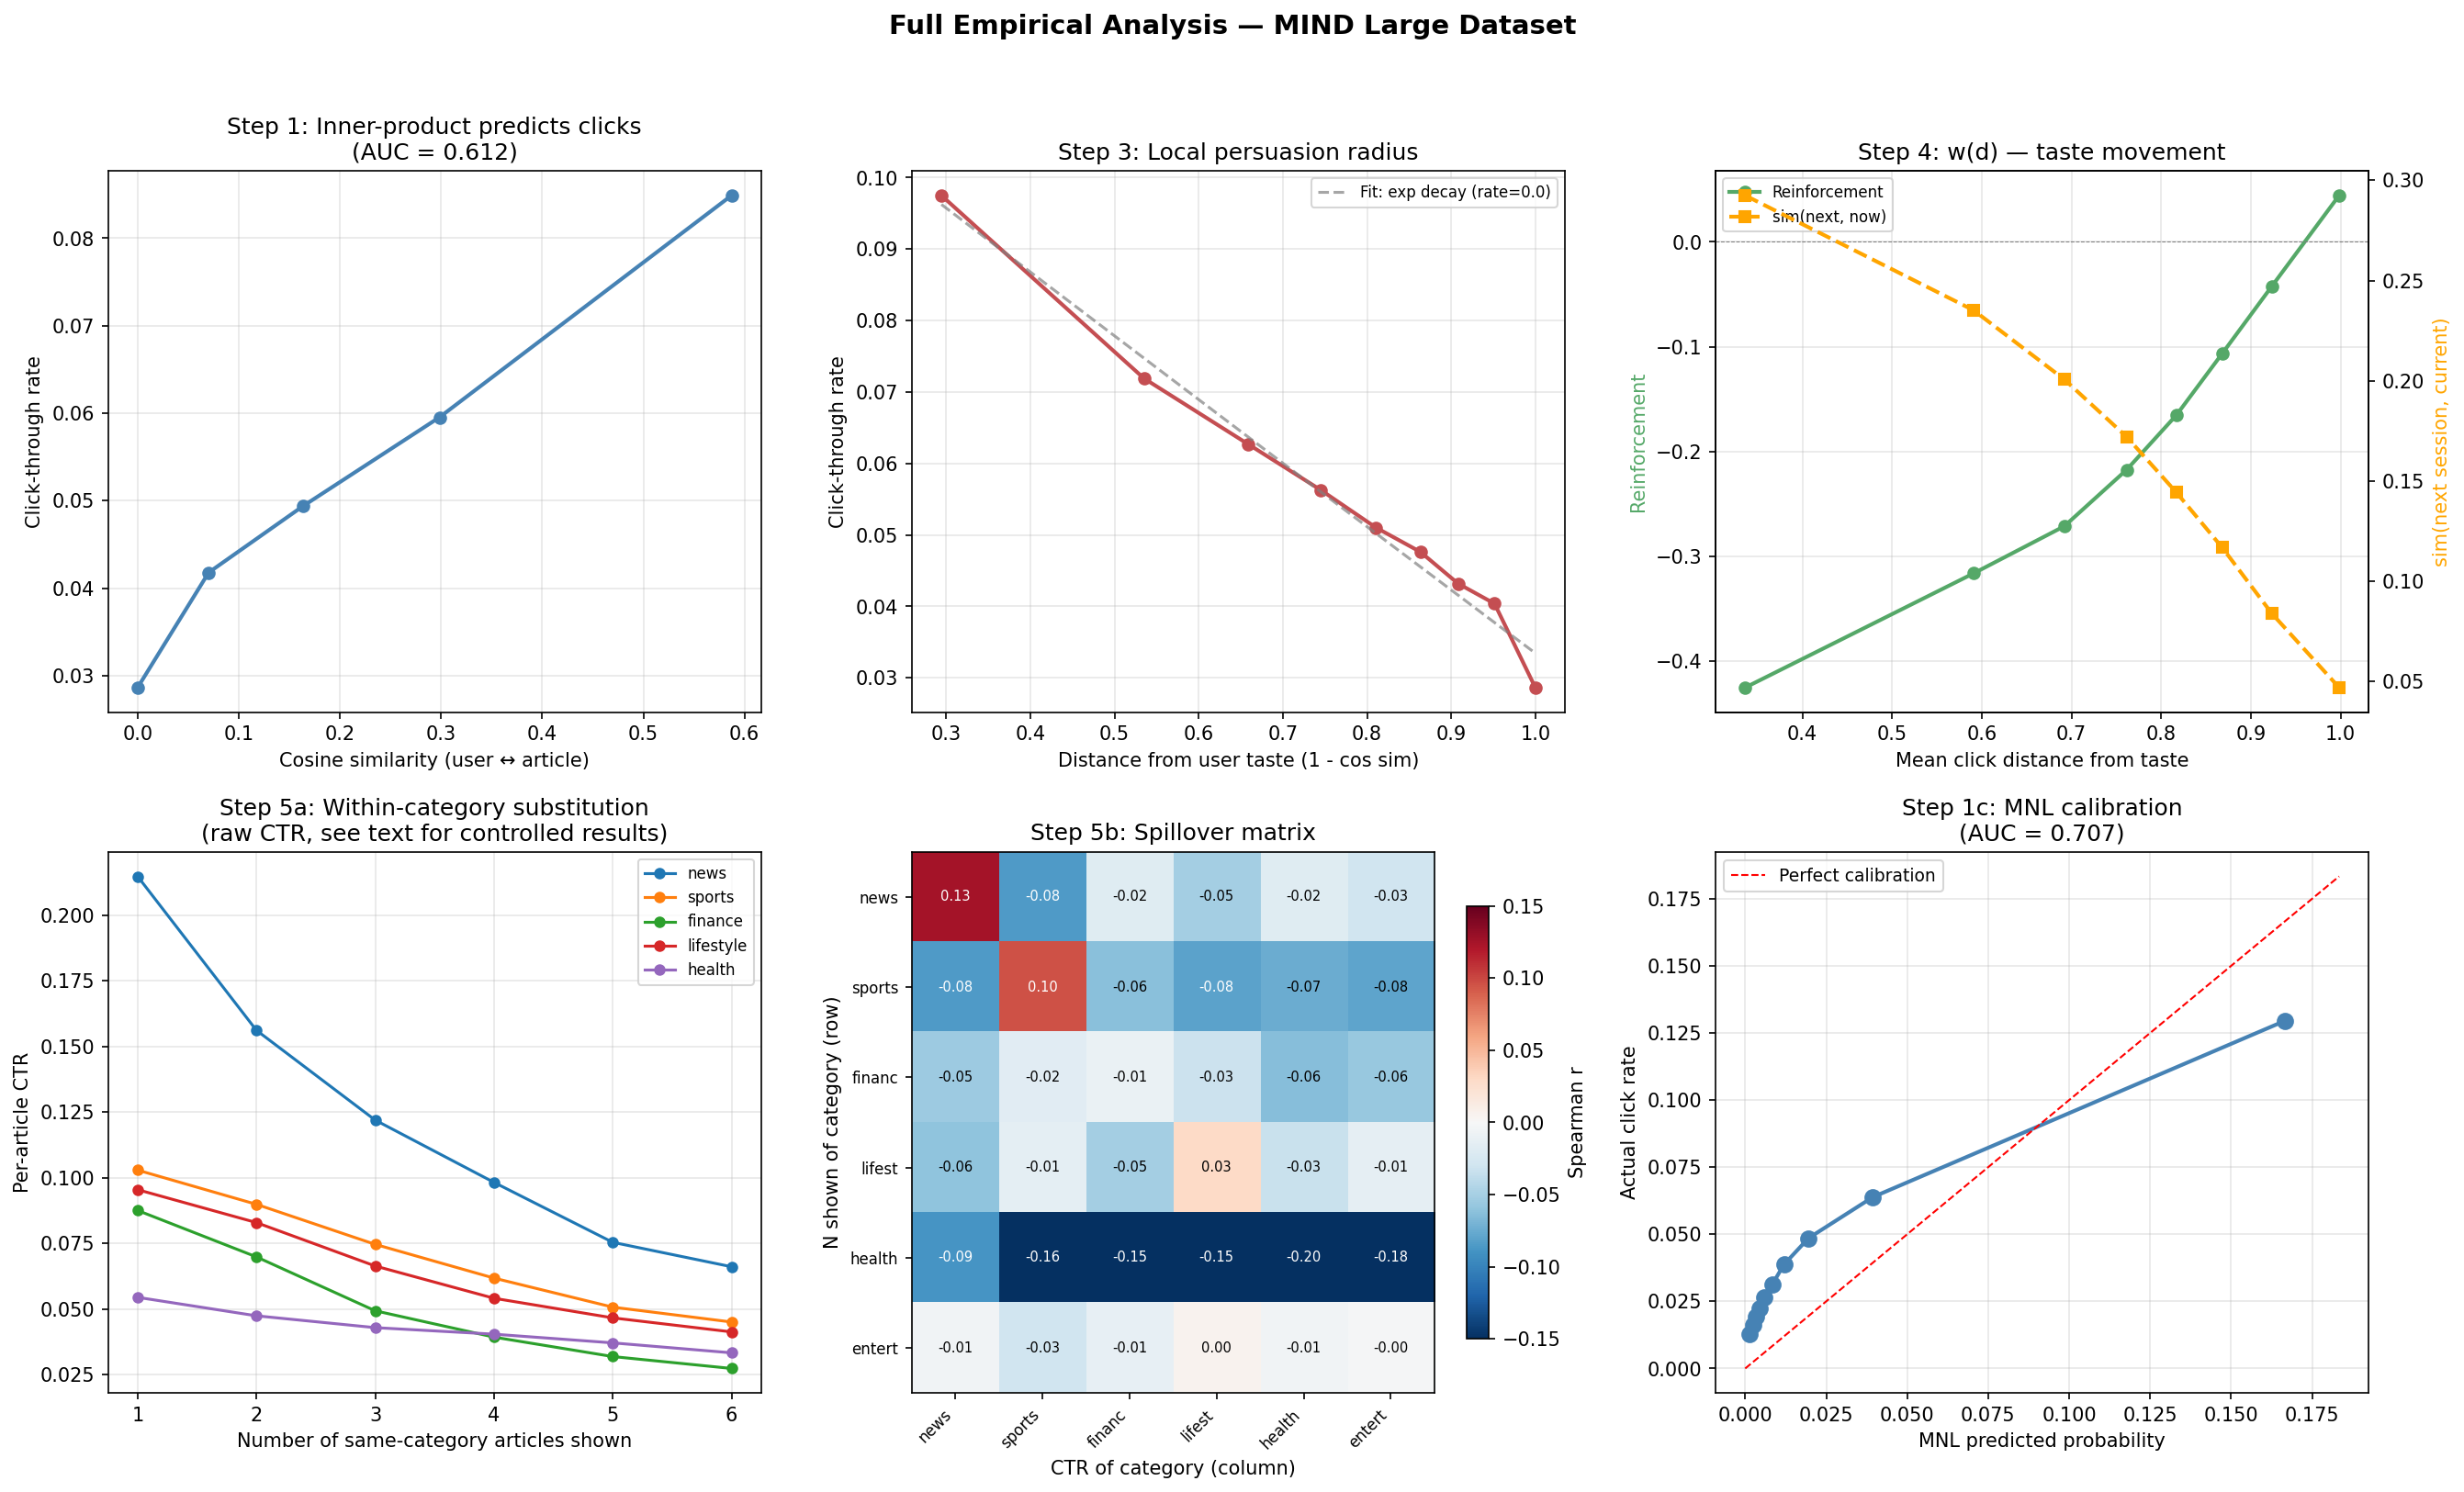
\includegraphics[width=\textwidth]{full_analysis.png}
    \caption{\textbf{(a)}~Cosine similarity vs.\ CTR. \textbf{(b)}~MNL calibration. \textbf{(c)}~CTR decay with distance. \textbf{(d)}~Reinforcement vs.\ click distance. \textbf{(e)}~Within-category substitution. \textbf{(f)}~Cross-category spillover heatmap.}
    \label{fig:full}
\end{figure}
\FloatBarrier

\begin{figure}[ht]
    \centering
    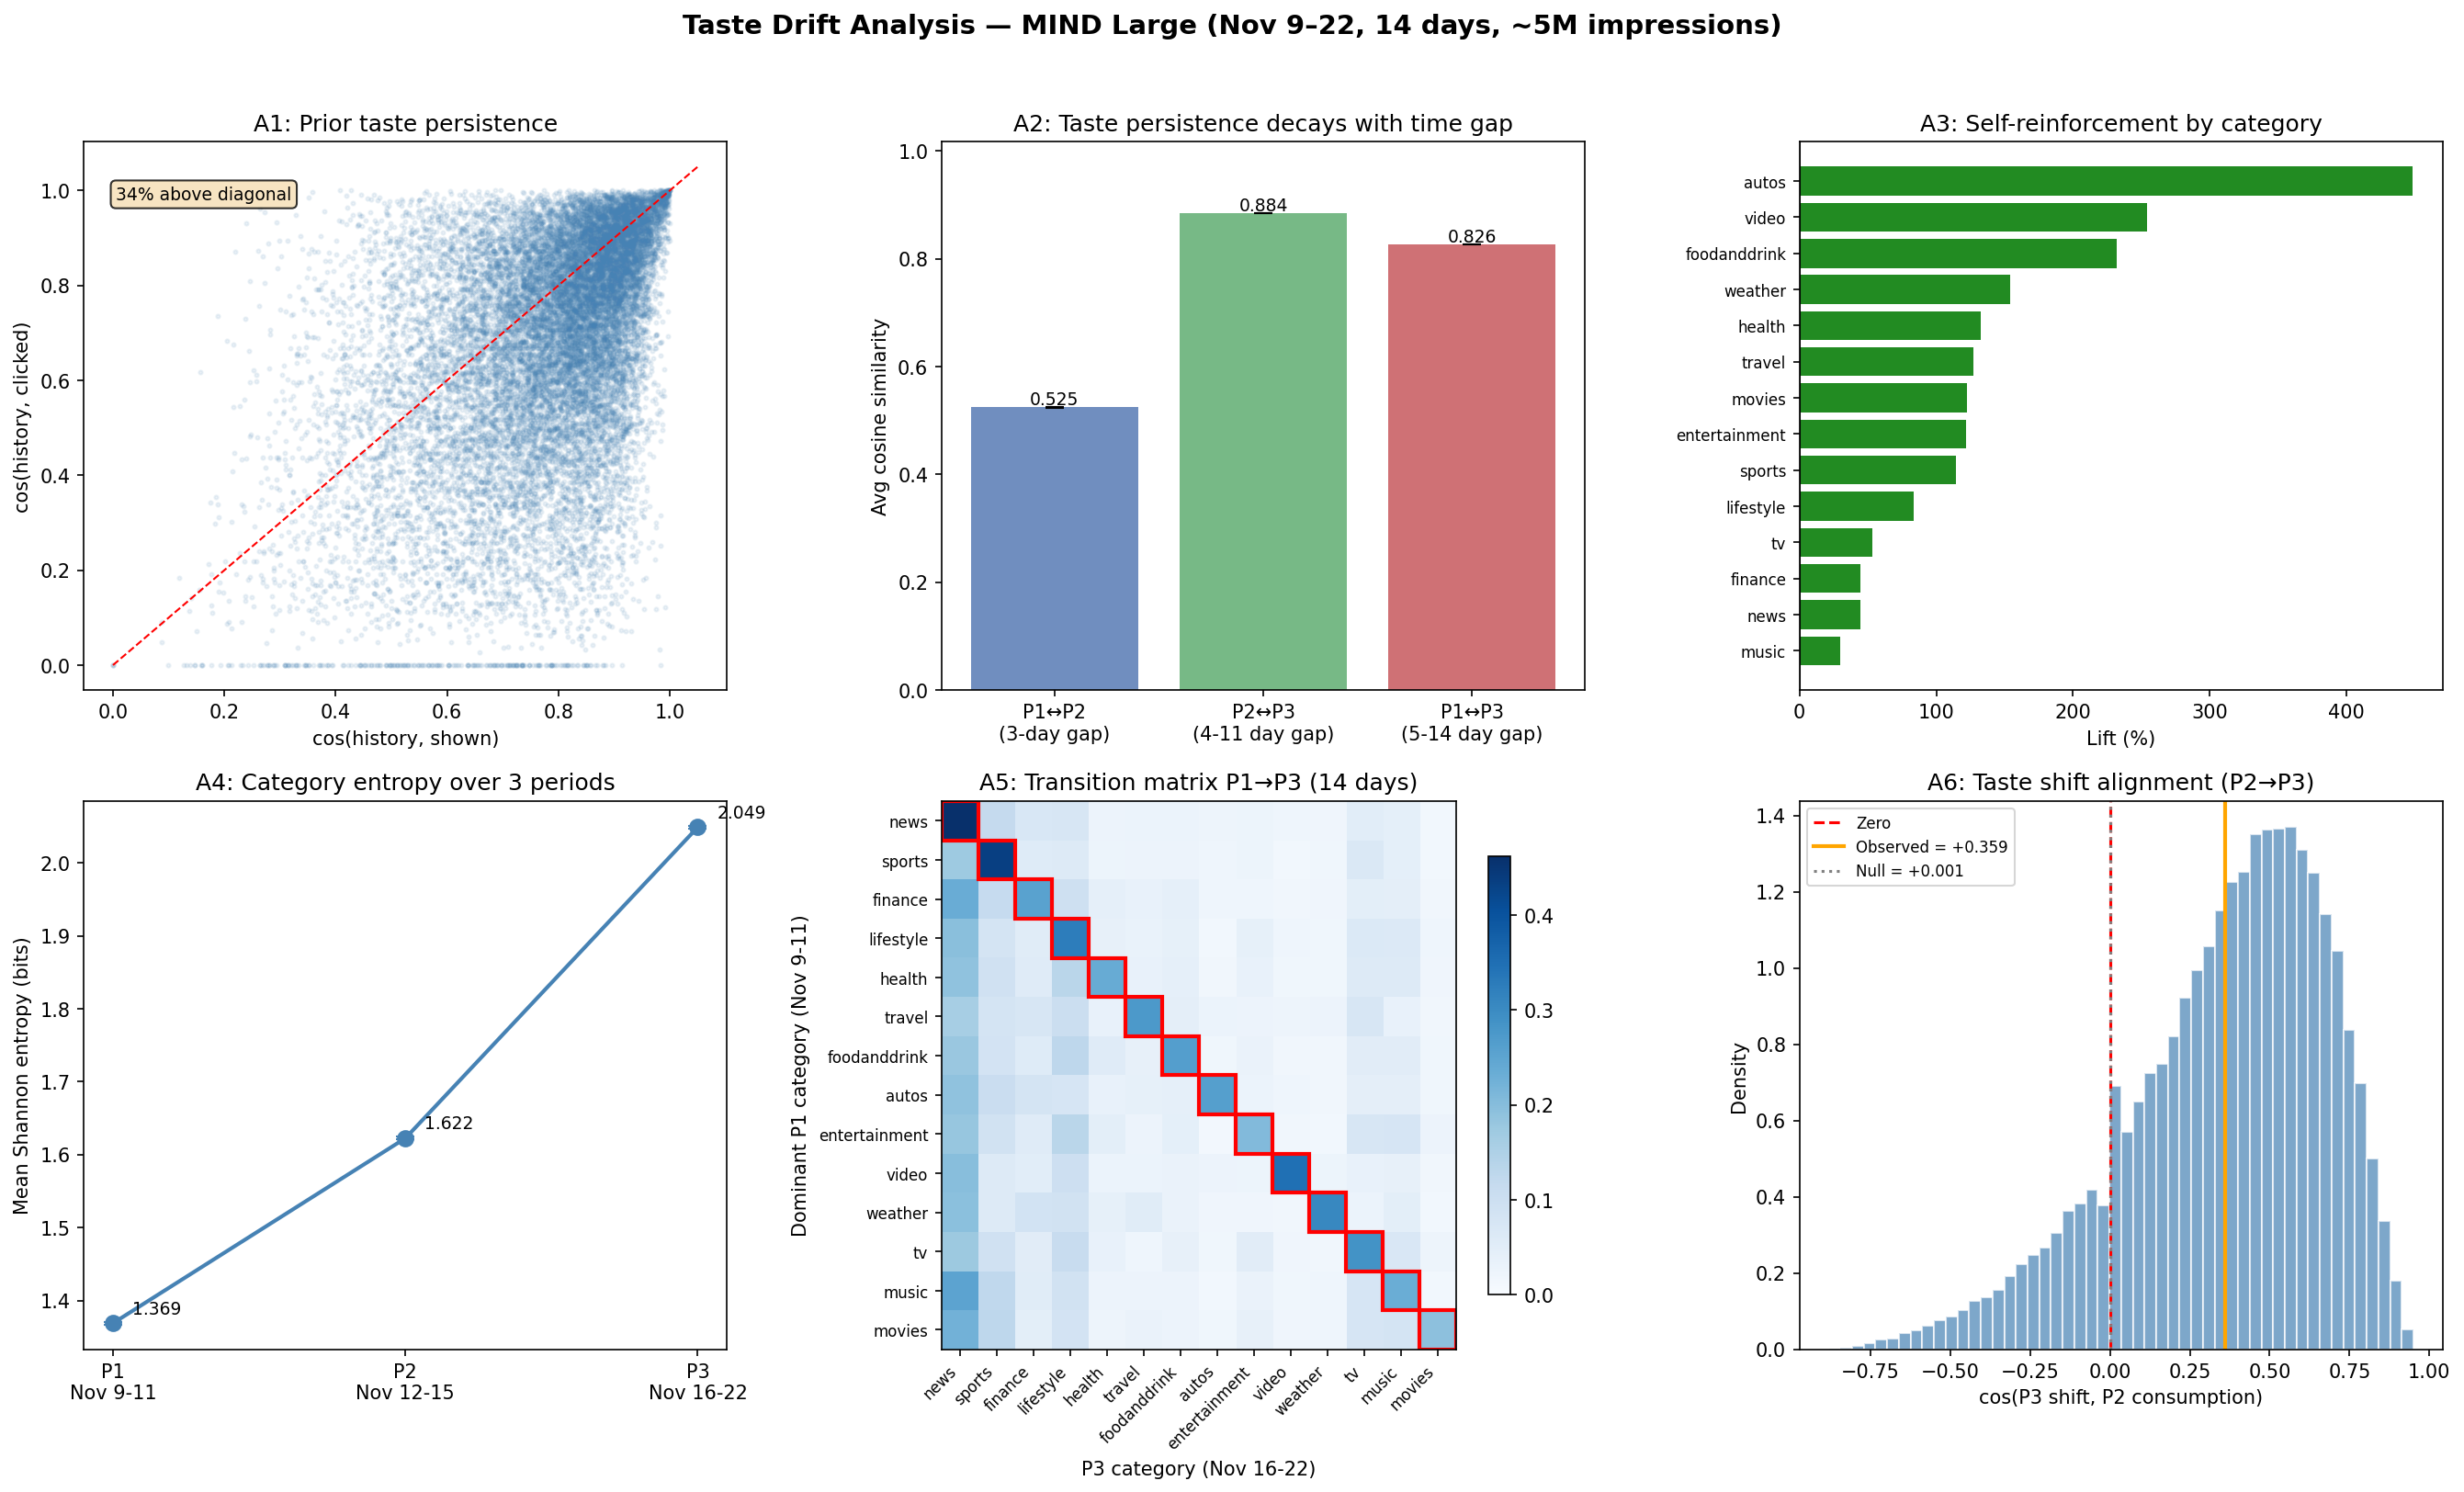
\includegraphics[width=\textwidth]{../output_large/taste_drift_large.png}
    \caption{Taste dynamics. \textbf{(A1)}~Prior taste persistence. \textbf{(A2)}~Similarity decay. \textbf{(A3)}~Self-reinforcement by category. \textbf{(A4)}~Entropy trajectory. \textbf{(A5)}~Transition heatmap. \textbf{(A6)}~Taste shift alignment vs.\ permutation null.}
    \label{fig:drift}
\end{figure}
\FloatBarrier

\begin{figure}[ht]
    \centering
    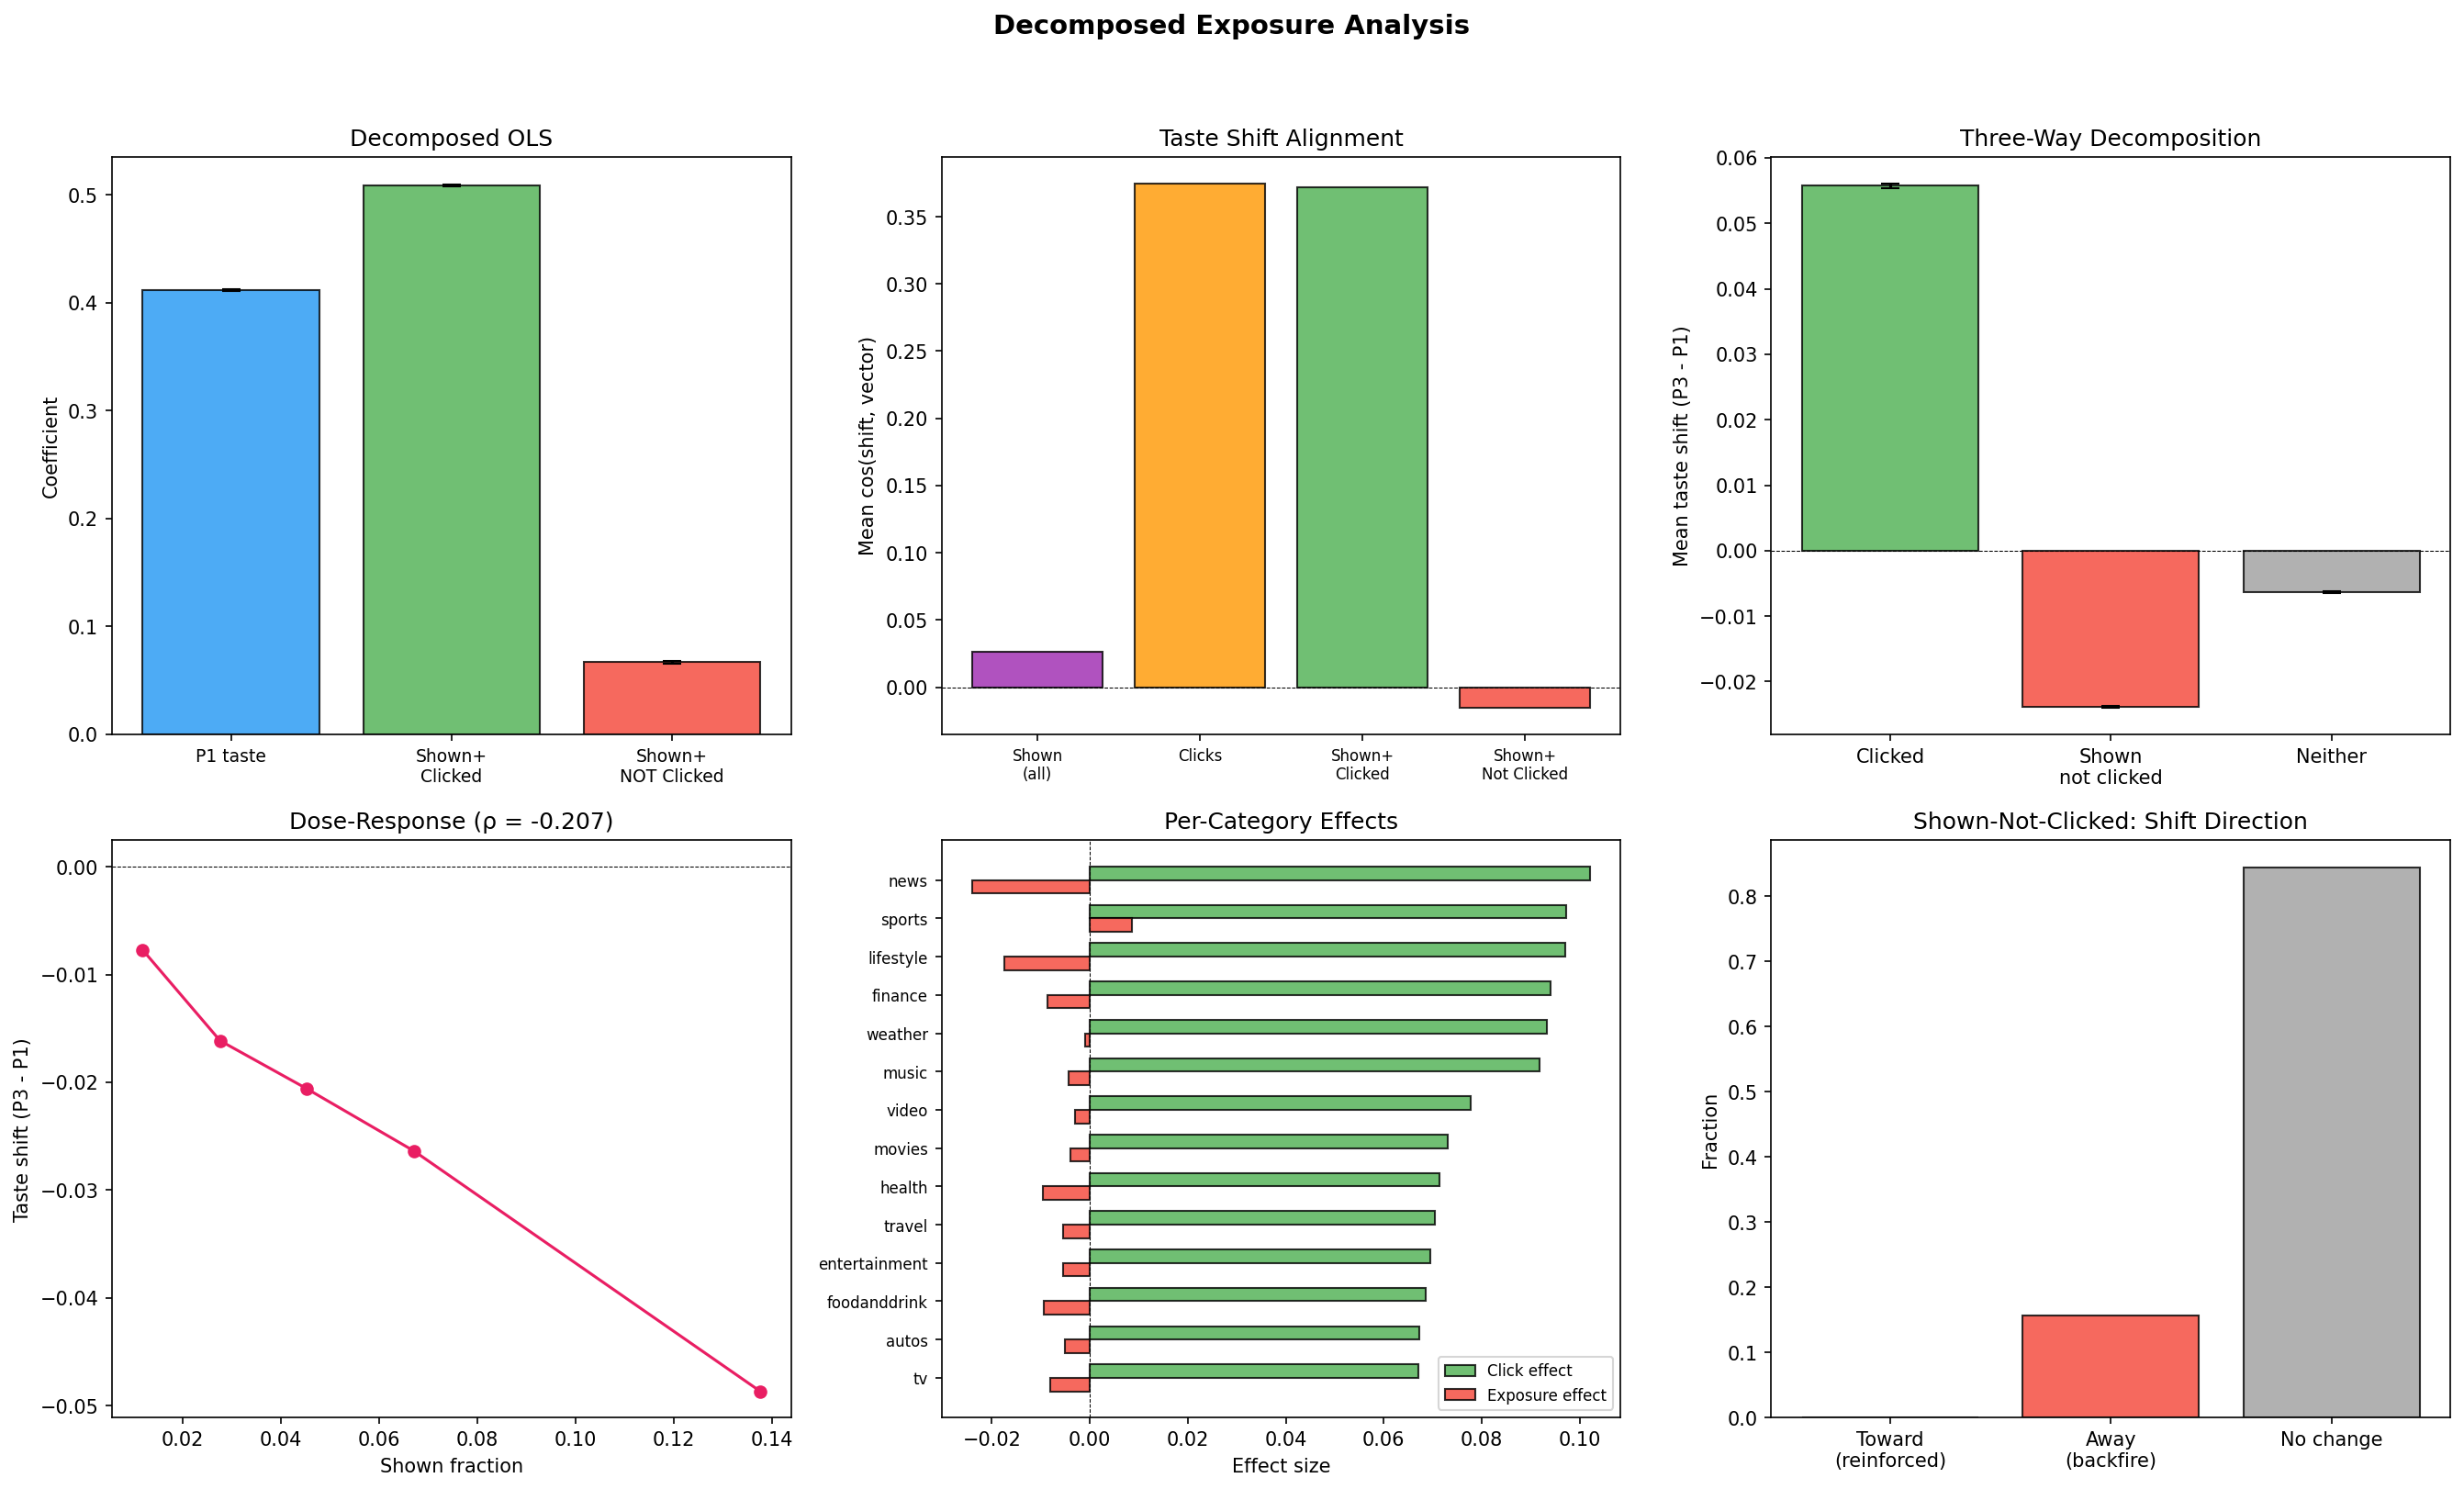
\includegraphics[width=\textwidth]{decomposed_exposure.png}
    \caption{Exposure vs.\ engagement. \textbf{(1)}~Decomposed OLS coefficients. \textbf{(2)}~Four-way cosine alignment. \textbf{(3)}~Three-way taste shift decomposition. \textbf{(4)}~Quintile dose-response. \textbf{(5)}~Per-category click vs.\ exposure effects. \textbf{(6)}~Direction of taste shift for shown-not-clicked pairs.}
    \label{fig:exposure}
\end{figure}
\FloatBarrier

\begin{figure}[ht]
    \centering
    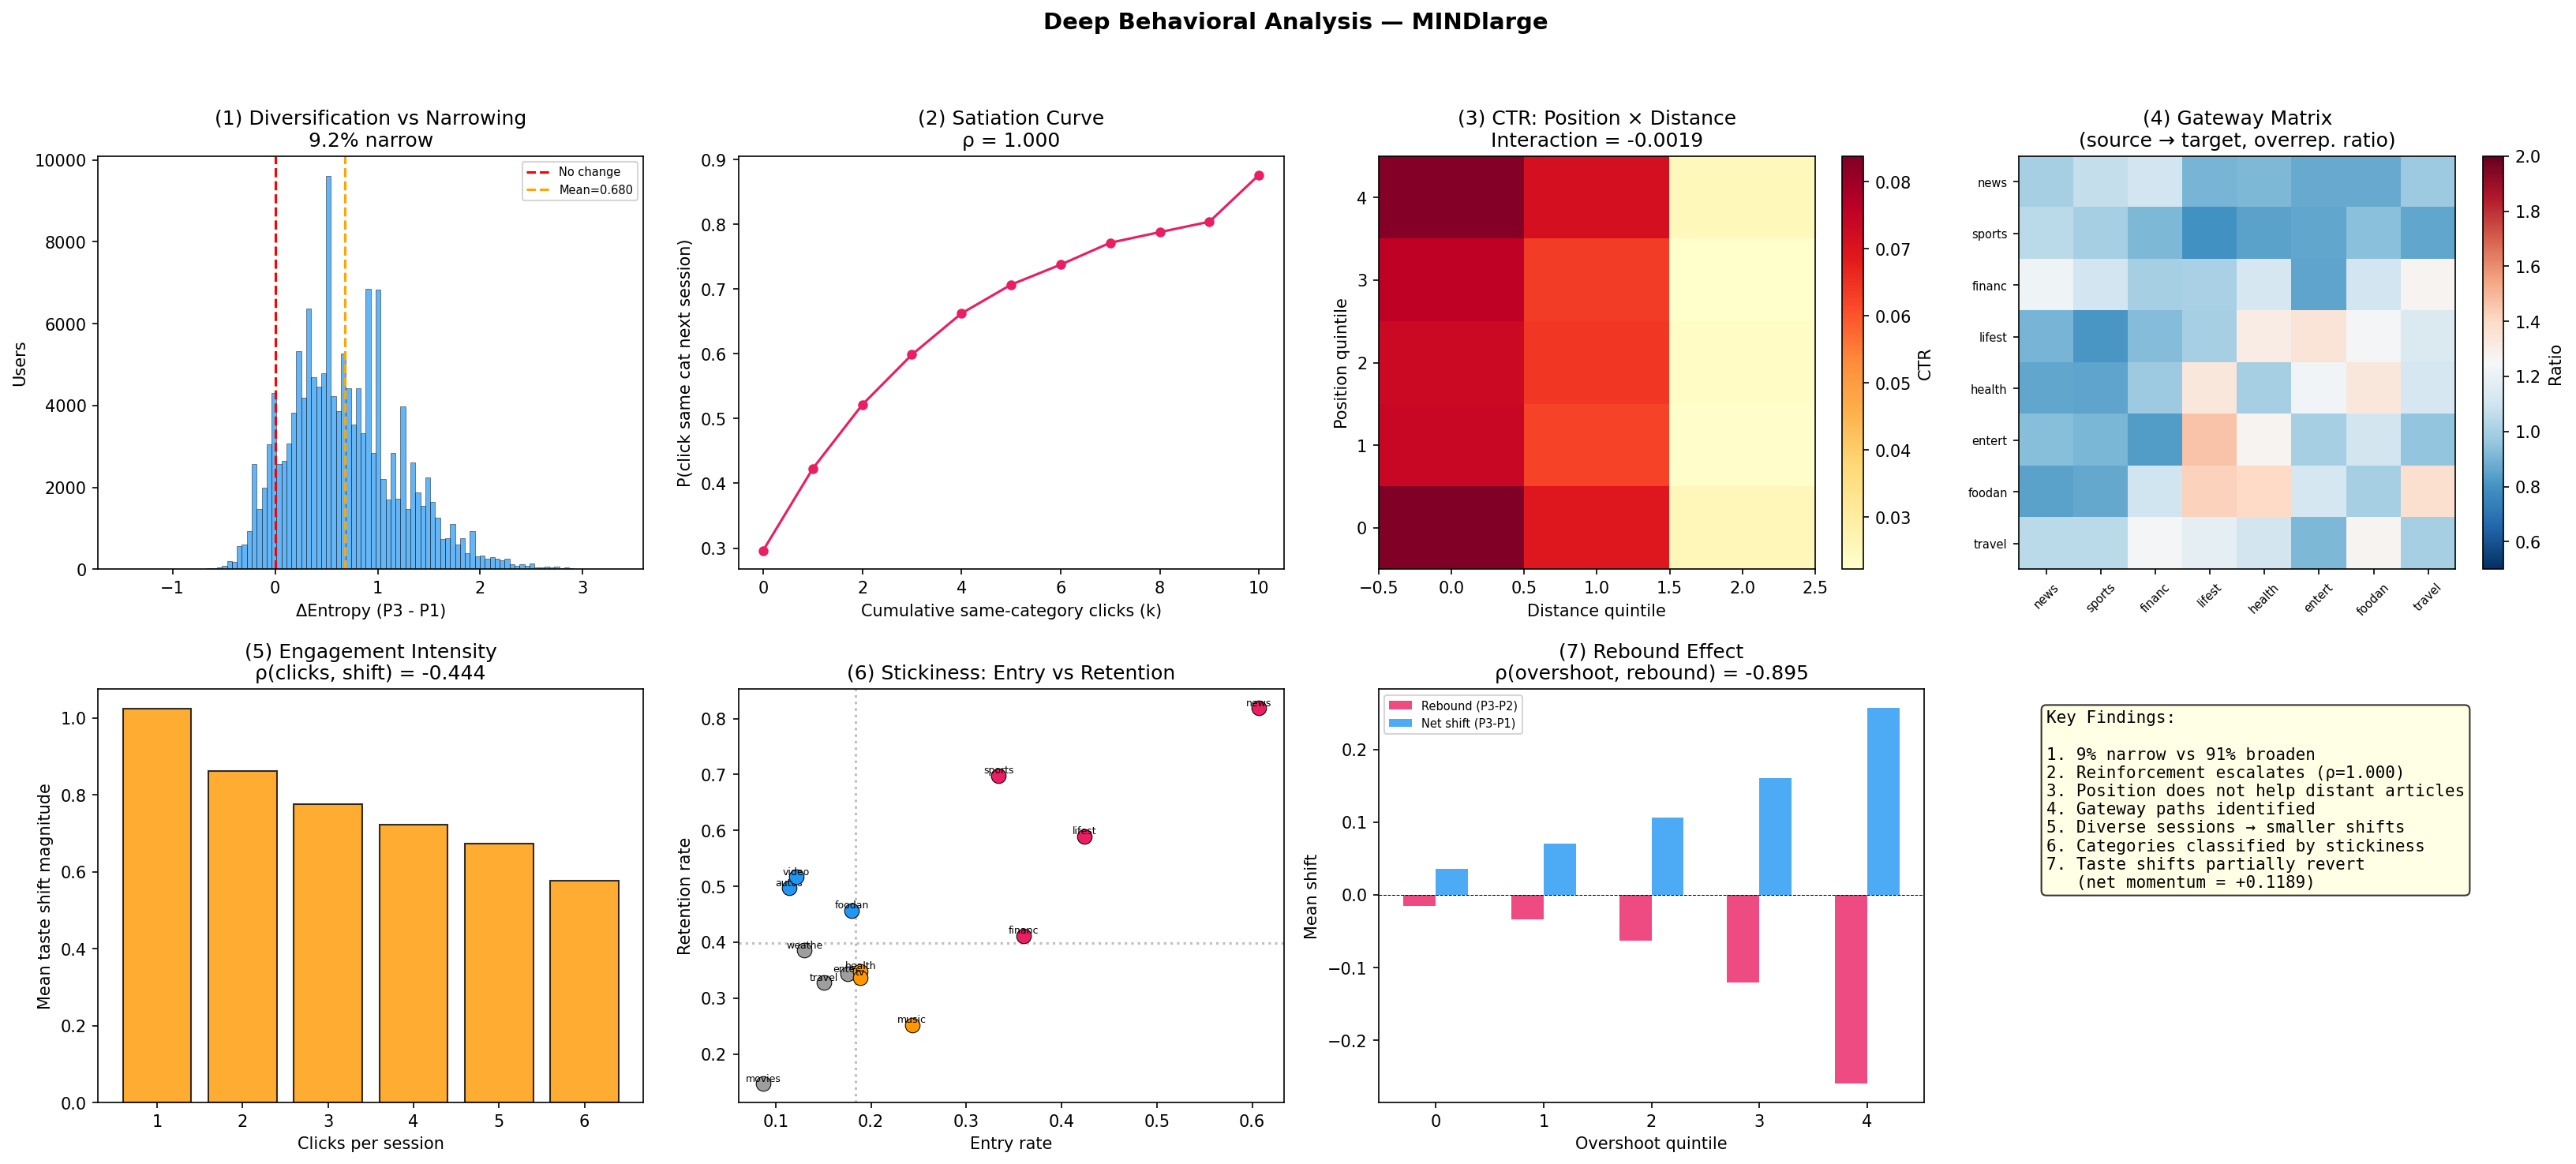
\includegraphics[width=\textwidth]{../output_large/deep_behavioral.png}
    \caption{Fine structure. \textbf{(1)}~Entropy change distribution. \textbf{(2)}~Satiation curves. \textbf{(3)}~Position $\times$ distance heatmap. \textbf{(4)}~Gateway network. \textbf{(5)}~Shift magnitude by session size. \textbf{(6)}~Entry vs.\ retention. \textbf{(7)}~Overshoot vs.\ reversion. \textbf{(8)}~Summary.}
    \label{fig:deep}
\end{figure}
\FloatBarrier


\end{document}
